
{
\begin{figure*}[th]
\begin{minipage}{\figWidthSix}
\begin{center}
\centerline{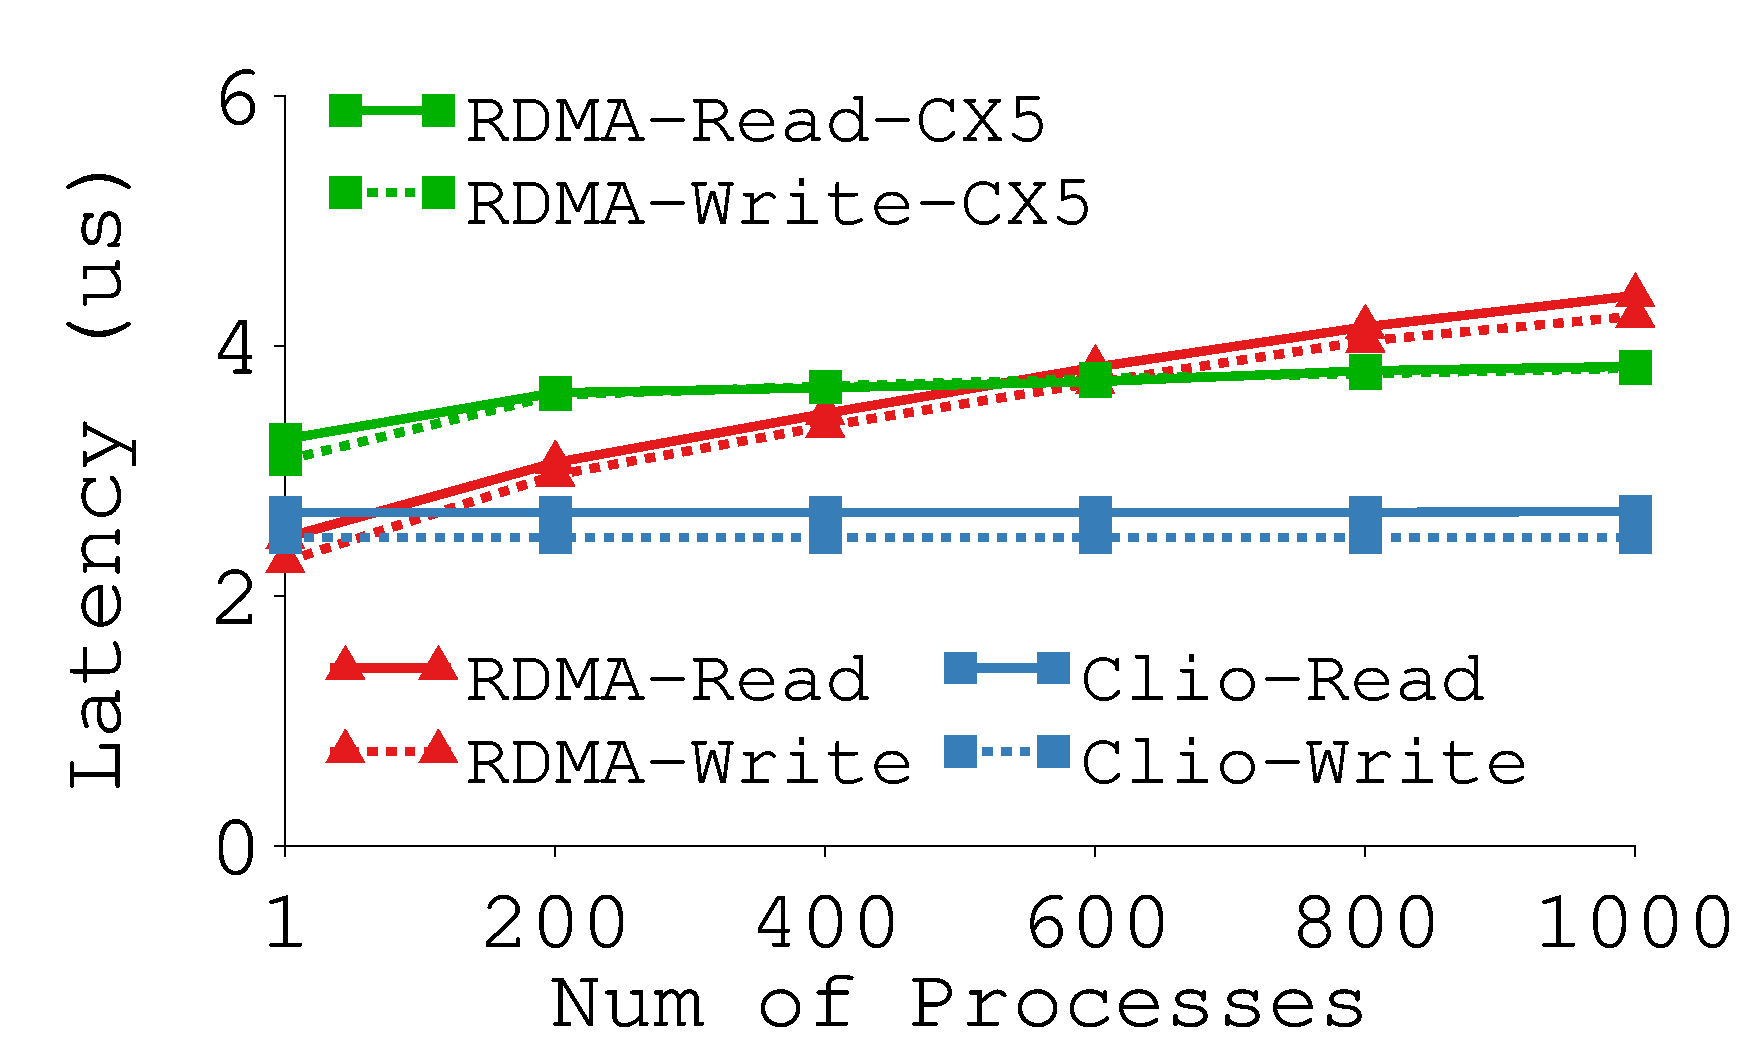
\includegraphics[width=\columnwidth]{Figures/g_plot_scalability_conn.pdf}}
\vspace{-0.1in}
\captionsetup{width=.9\columnwidth}
\mycaption{fig-conn}{Process (Connection) Scalability.}
{
}
\end{center}
\end{minipage}
%\begin{minipage}{0.01in}
%\hspace{0.01in}
%\end{minipage}
\begin{minipage}{\figWidthSix}
\begin{center}
\centerline{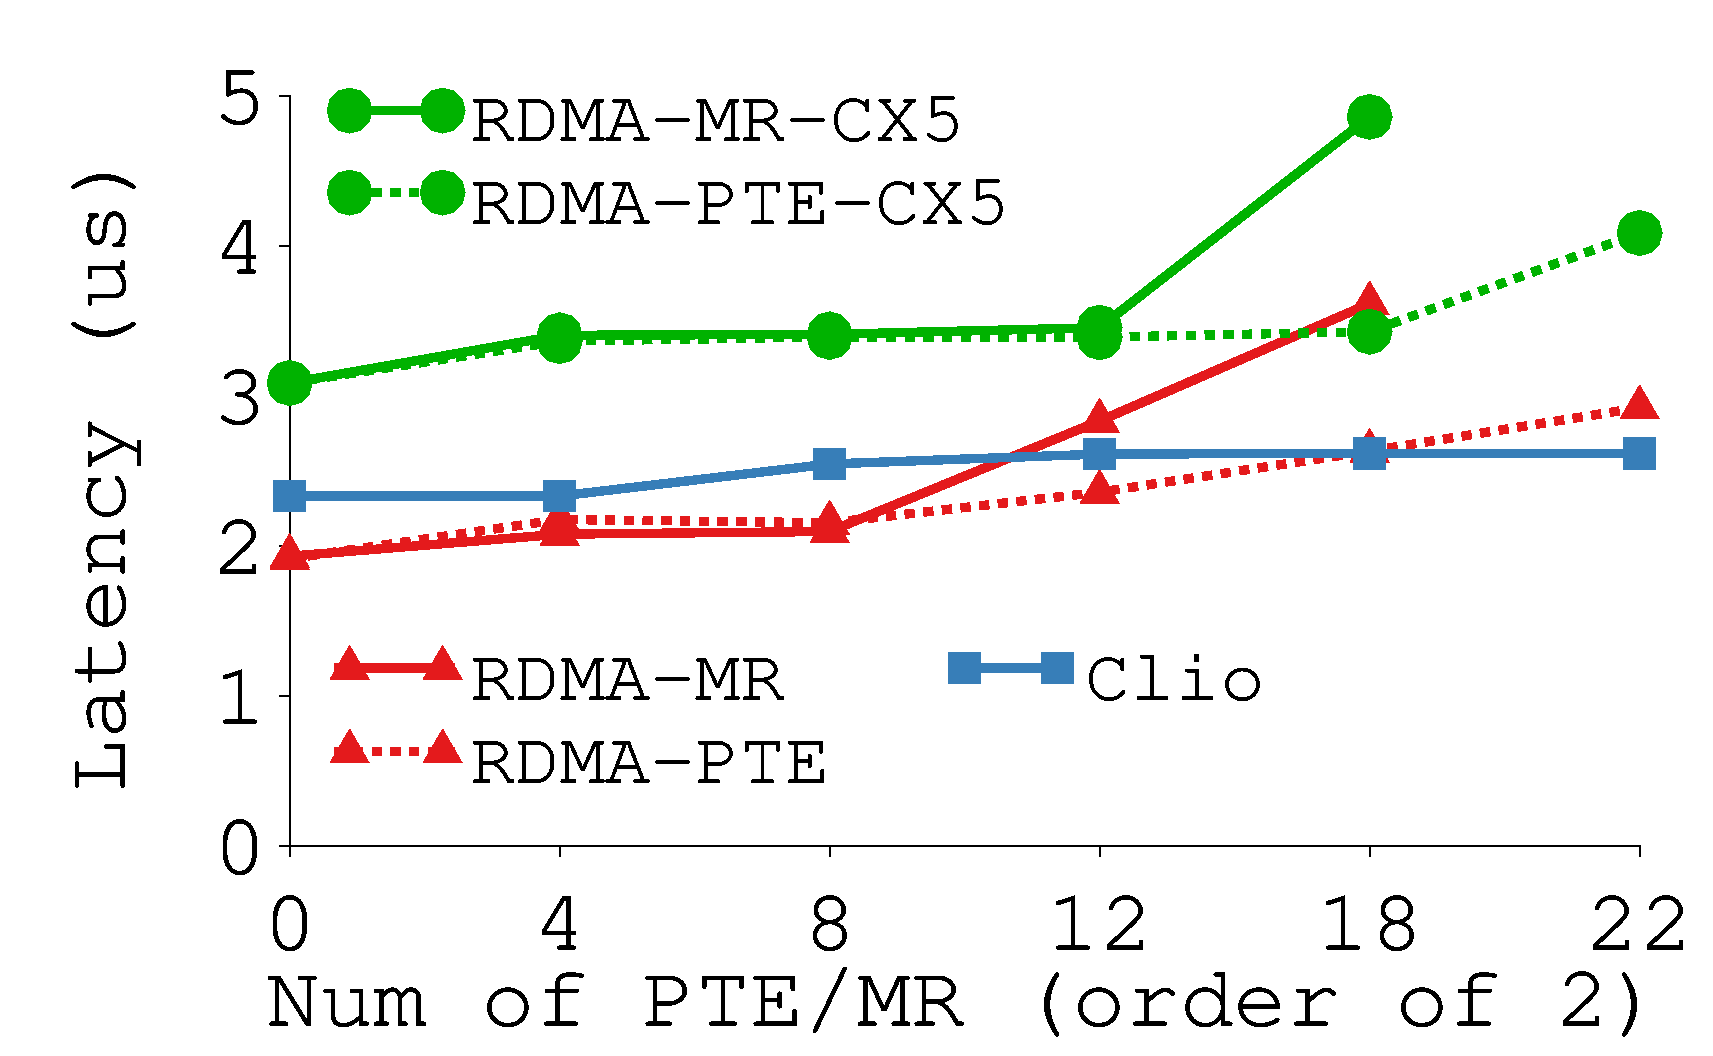
\includegraphics[width=\columnwidth]{Figures/g_plot_scalability_pte.pdf}}
\vspace{-0.1in}
\captionsetup{width=.9\columnwidth}
\mycaption{fig-pte-mr}{PTE and MR Scalability.}
{
RDMA fails beyond $2^{18}$ MRs. 
}
\end{center}
\end{minipage}
%\begin{minipage}{0.01in}
%\hspace{0.01in}
%\end{minipage}
\begin{minipage}{\figWidthSix}
\begin{center}
\centerline{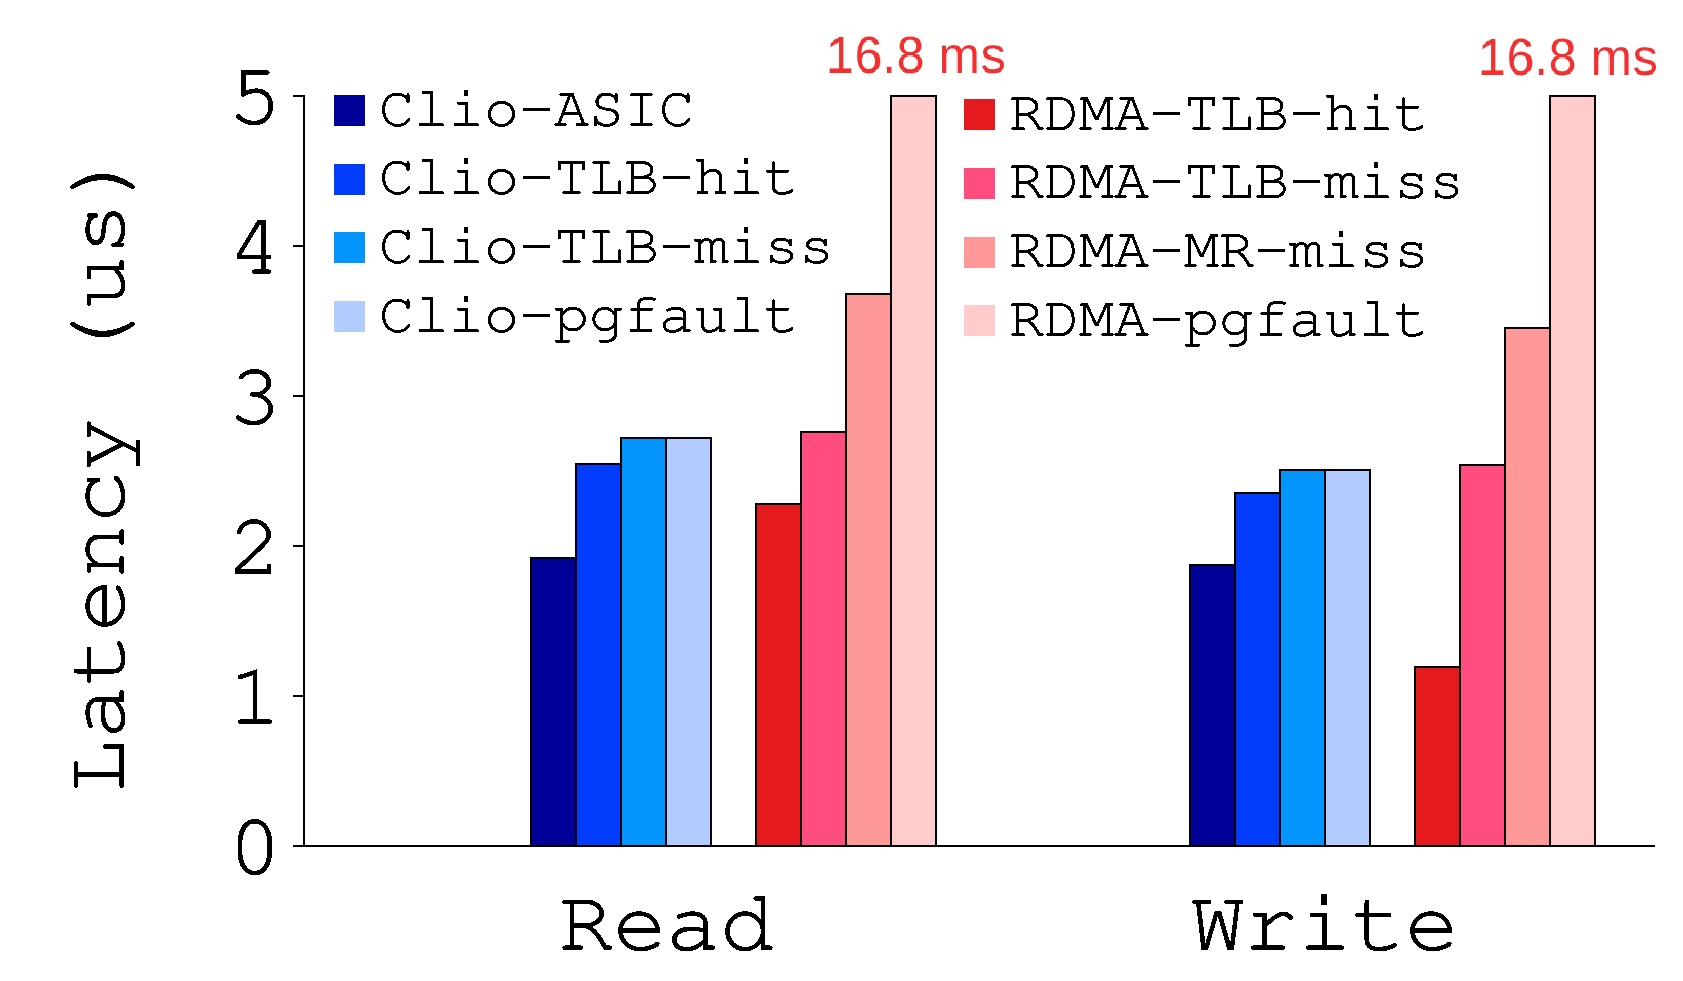
\includegraphics[width=\columnwidth]{Figures/g_plot_latency_comparison.pdf}}
\vspace{-0.1in}
\captionsetup{width=.9\columnwidth}
\mycaption{fig-miss-hit}{Comparison of TLB Miss and page fault.}
{
\sys-ASIC are projected values of TLB hit.
}
\end{center}
\end{minipage}
\begin{minipage}{\figWidthSix}
\begin{center}
\centerline{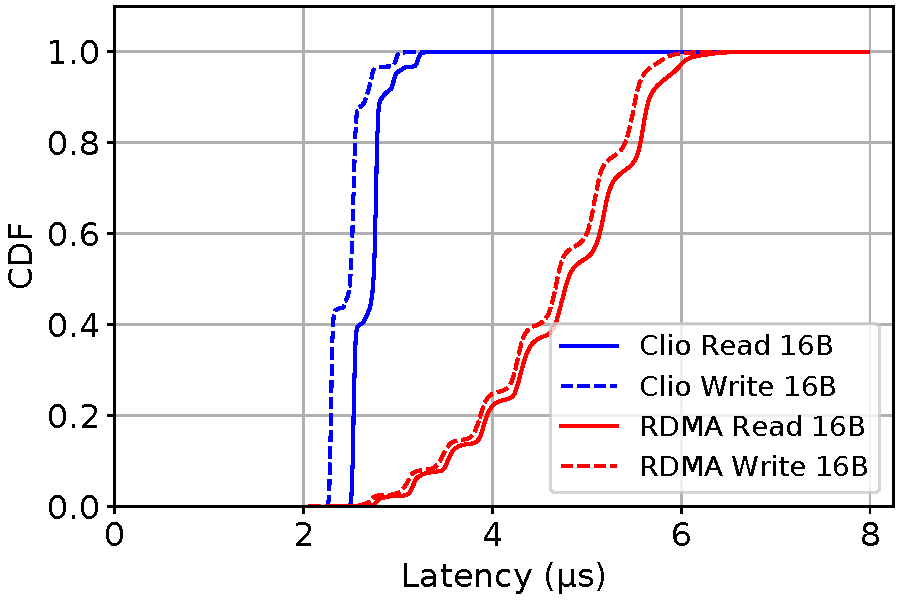
\includegraphics[width=\columnwidth]{Figures/clio_rdma_lat_cdf.pdf}}
\vspace{-0.1in}
\captionsetup{width=.9\columnwidth}
\mycaption{fig-tail-latency}{Latency CDF.}
{
}
\end{center}
\end{minipage}
\vspace{-0.1in}
\end{figure*}
}

{
\begin{figure*}[th]
\begin{center}
\centerline{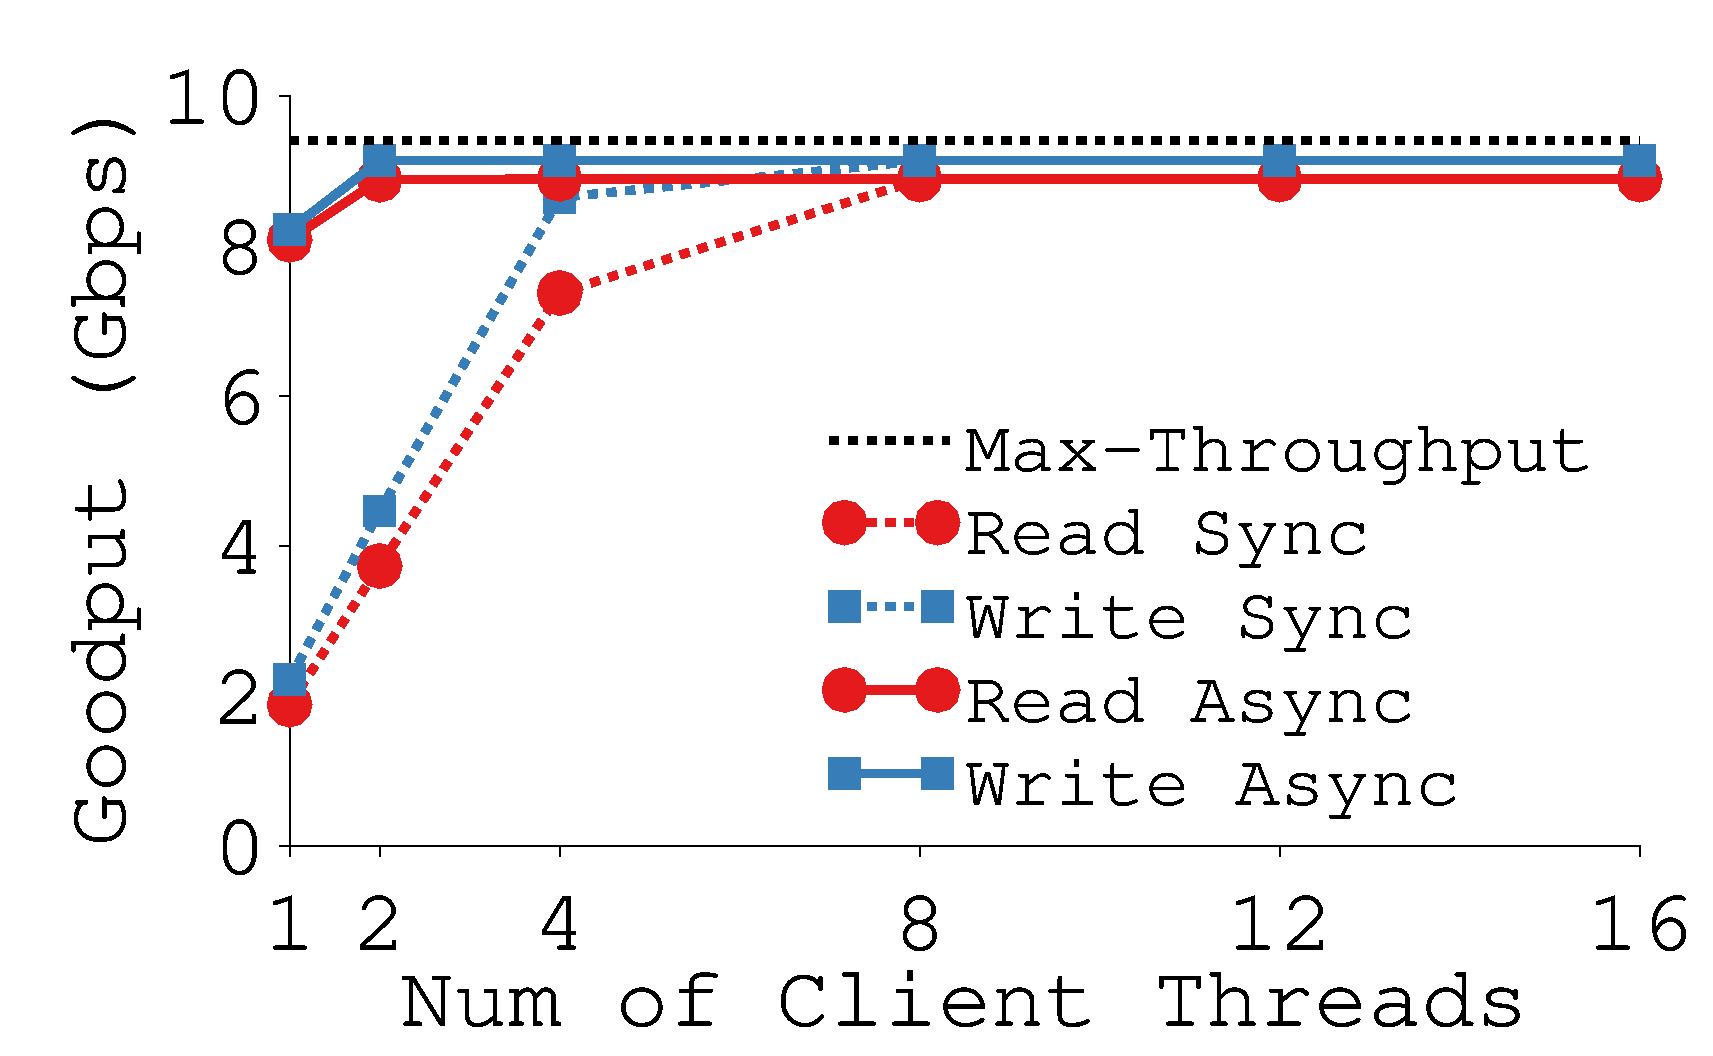
\includegraphics[width=0.5\textwidth]{clio/Figures/g_plot_throughput.pdf}}
\mycaption{fig-read-write-throughput}{End-to-End Goodput.}
{
1\KB\ requests. % between 1 \CN\ and 1 \MN.
}
\end{center}
\end{figure*}
}
{
\begin{figure*}[h]
\begin{center}
\centerline{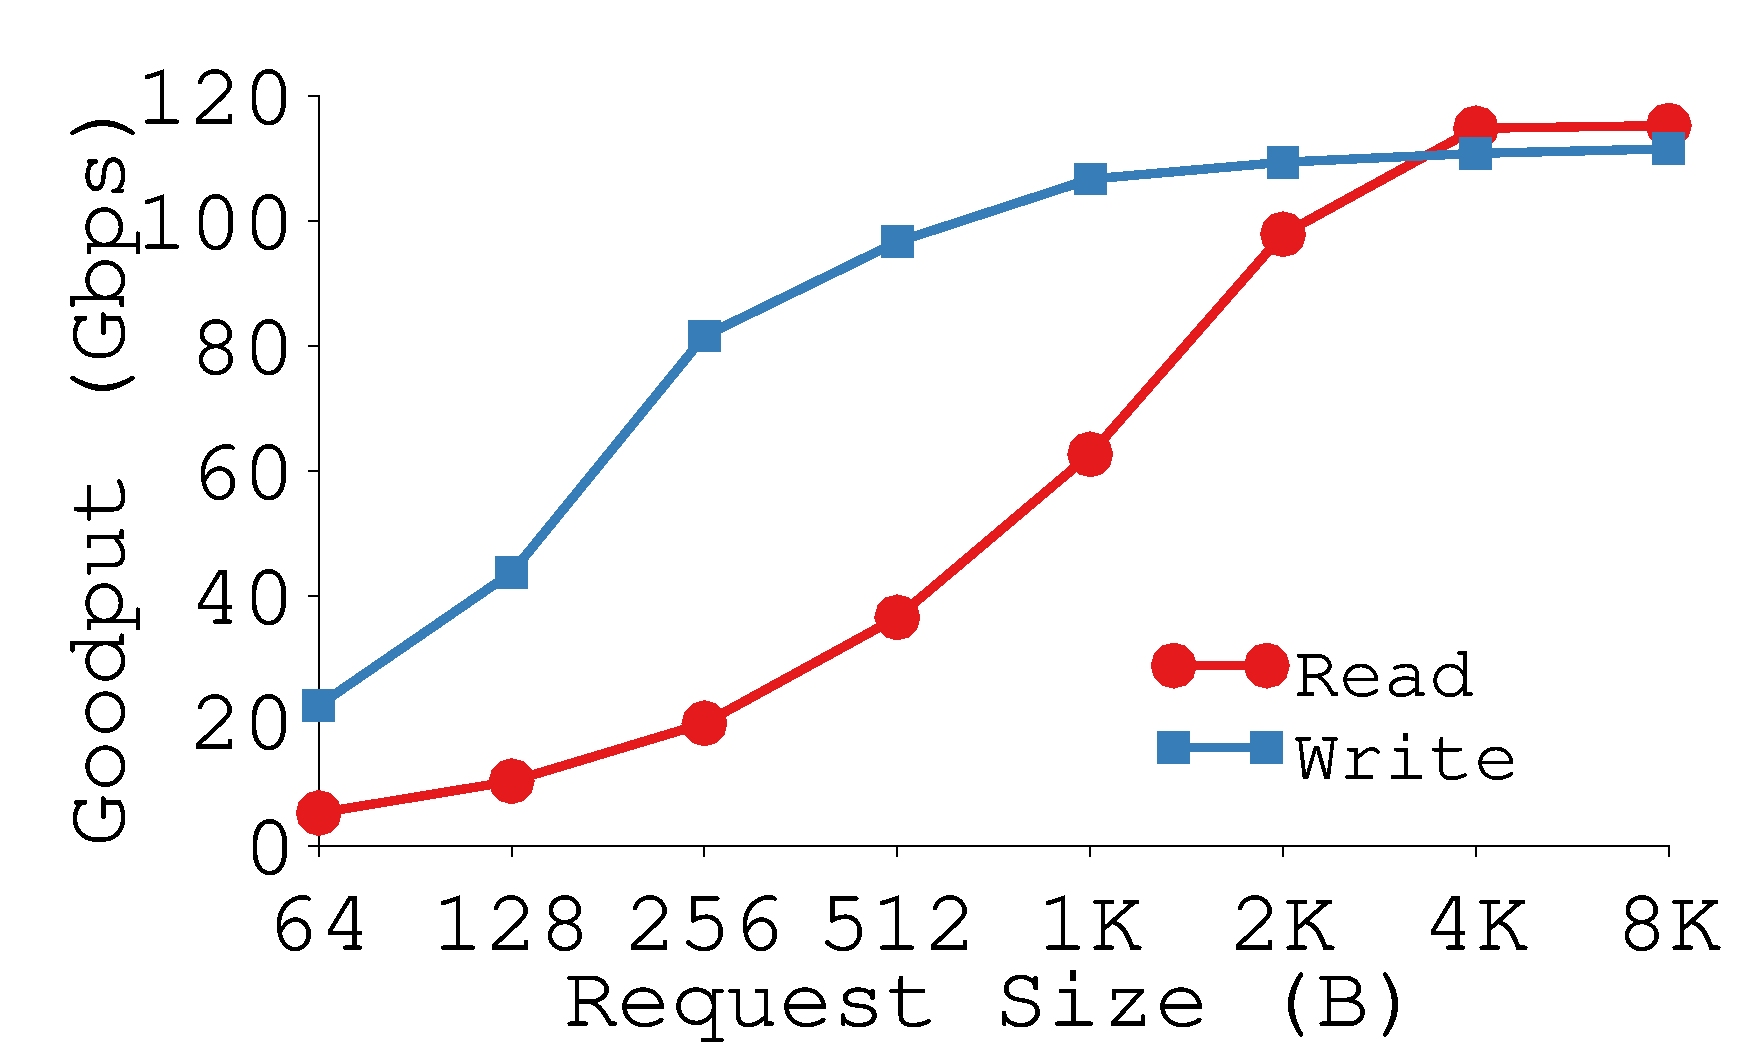
\includegraphics[width=0.5\textwidth]{clio/Figures/g_plot_onboard_throughput.pdf}}
\mycaption{fig-onboard-throughput}{On-board Goodput.}
{
FPGA test module generates requests at maximum speed.
}
\end{center}
\end{figure*}
}
{
\begin{figure*}[h]
\begin{center}
\centerline{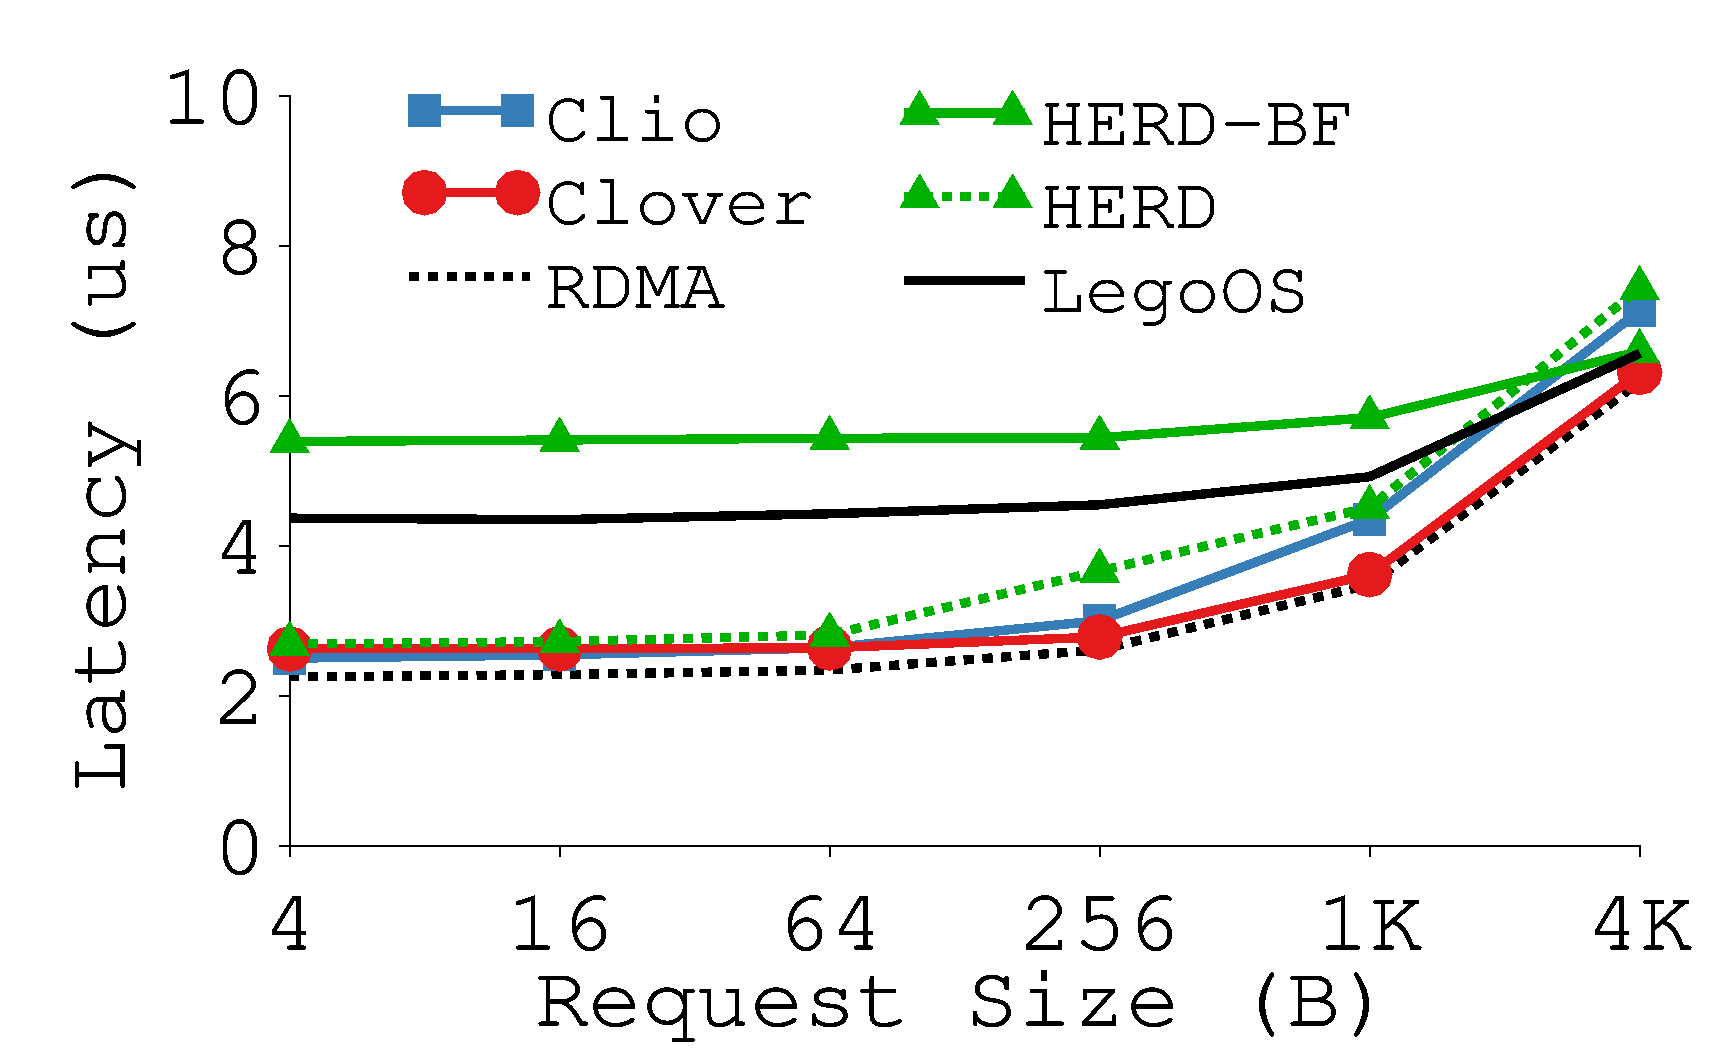
\includegraphics[width=0.5\textwidth]{clio/Figures/g_plot_read_latency.pdf}}
\mycaption{fig-read-lat}{Read Latency.}
{
HERD-BF: HERD running on BlueField. %SmartNIC.
}
\end{center}
\end{figure*}
}
{
\begin{figure*}[h]
\begin{center}
\centerline{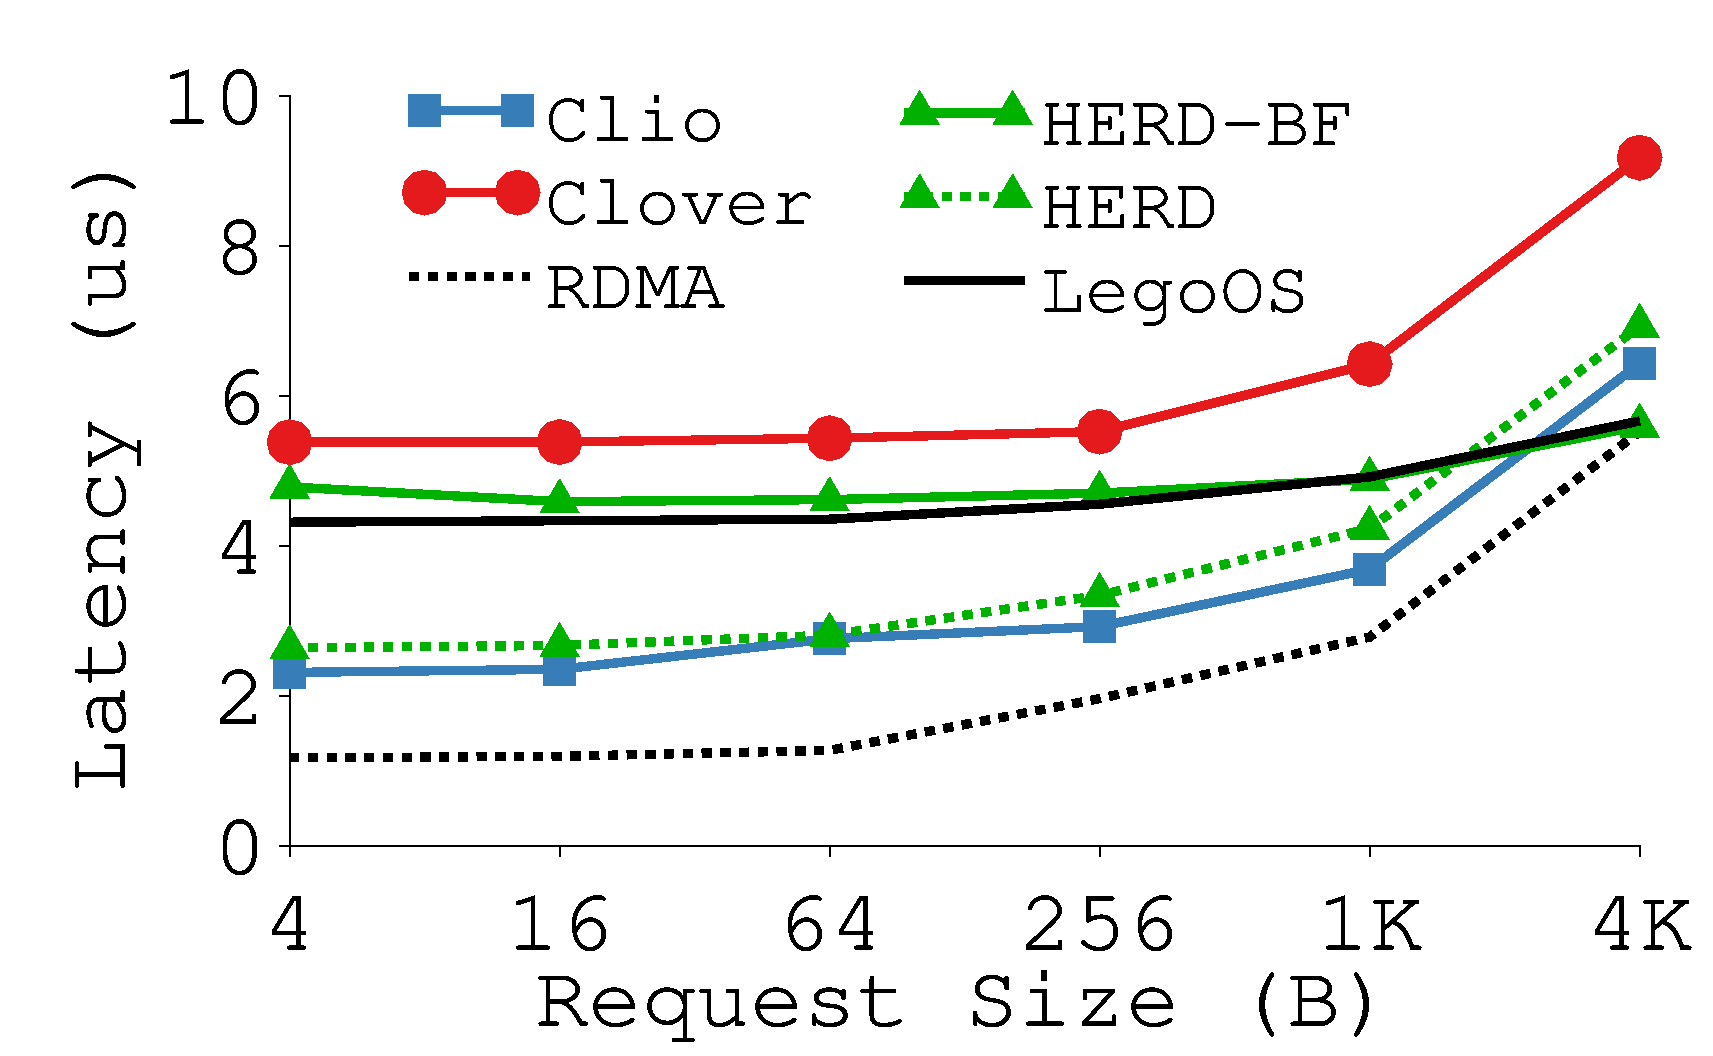
\includegraphics[width=0.5\textwidth]{clio/Figures/g_plot_write_latency.pdf}}
\mycaption{fig-write-lat}{Write Latency.}
{
Clover requires $\ge$ 2 RTTs for write.
}
\end{center}
\end{figure*}
}

\section{Evaluation}
\label{sec:clio:results}


Our evaluation reveals the scalability, throughput, median and tail latency, energy and resource consumption of \sys.
%, and how it compares with state-of-the-art systems. 
We compare \sys's end-to-end performance with industry-grade NICs (ASIC) and well-tuned RDMA-based software systems.
All \sys's results are FPGA-based, which would be improved with ASIC implementation.
%Nonetheless, \sys\ significantly outperforms RDMA on scalability and tail latency, while being similar on other measurements.

\ulinebfpara{Environment.}
We evaluated \sys\ in our local cluster of four \CN{}s and four \MN{}s (Xilinx ZCU106 boards),
%\footnote{Unfortunately, our process of purchasing and setting up a bigger cluster was significantly delayed because of COVID-19},
all connected to an Nvidia 40\Gbps\ VPI switch.
Each \CN\ is a Dell PowerEdge R740 server equipped with a Xeon Gold 5128 CPU and a 40\Gbps\ Nvidia ConnectX-3 NIC,
with two of them also having an Nvidia BlueField SmartNIC~\cite{BlueField}.
We also include results from CloudLab~\cite{CloudLab} with the Nvidia ConnectX-5 NIC.


\subsection{Basic Microbenchmark Performance}

{
\begin{figure*}[th]
\begin{center}
\centerline{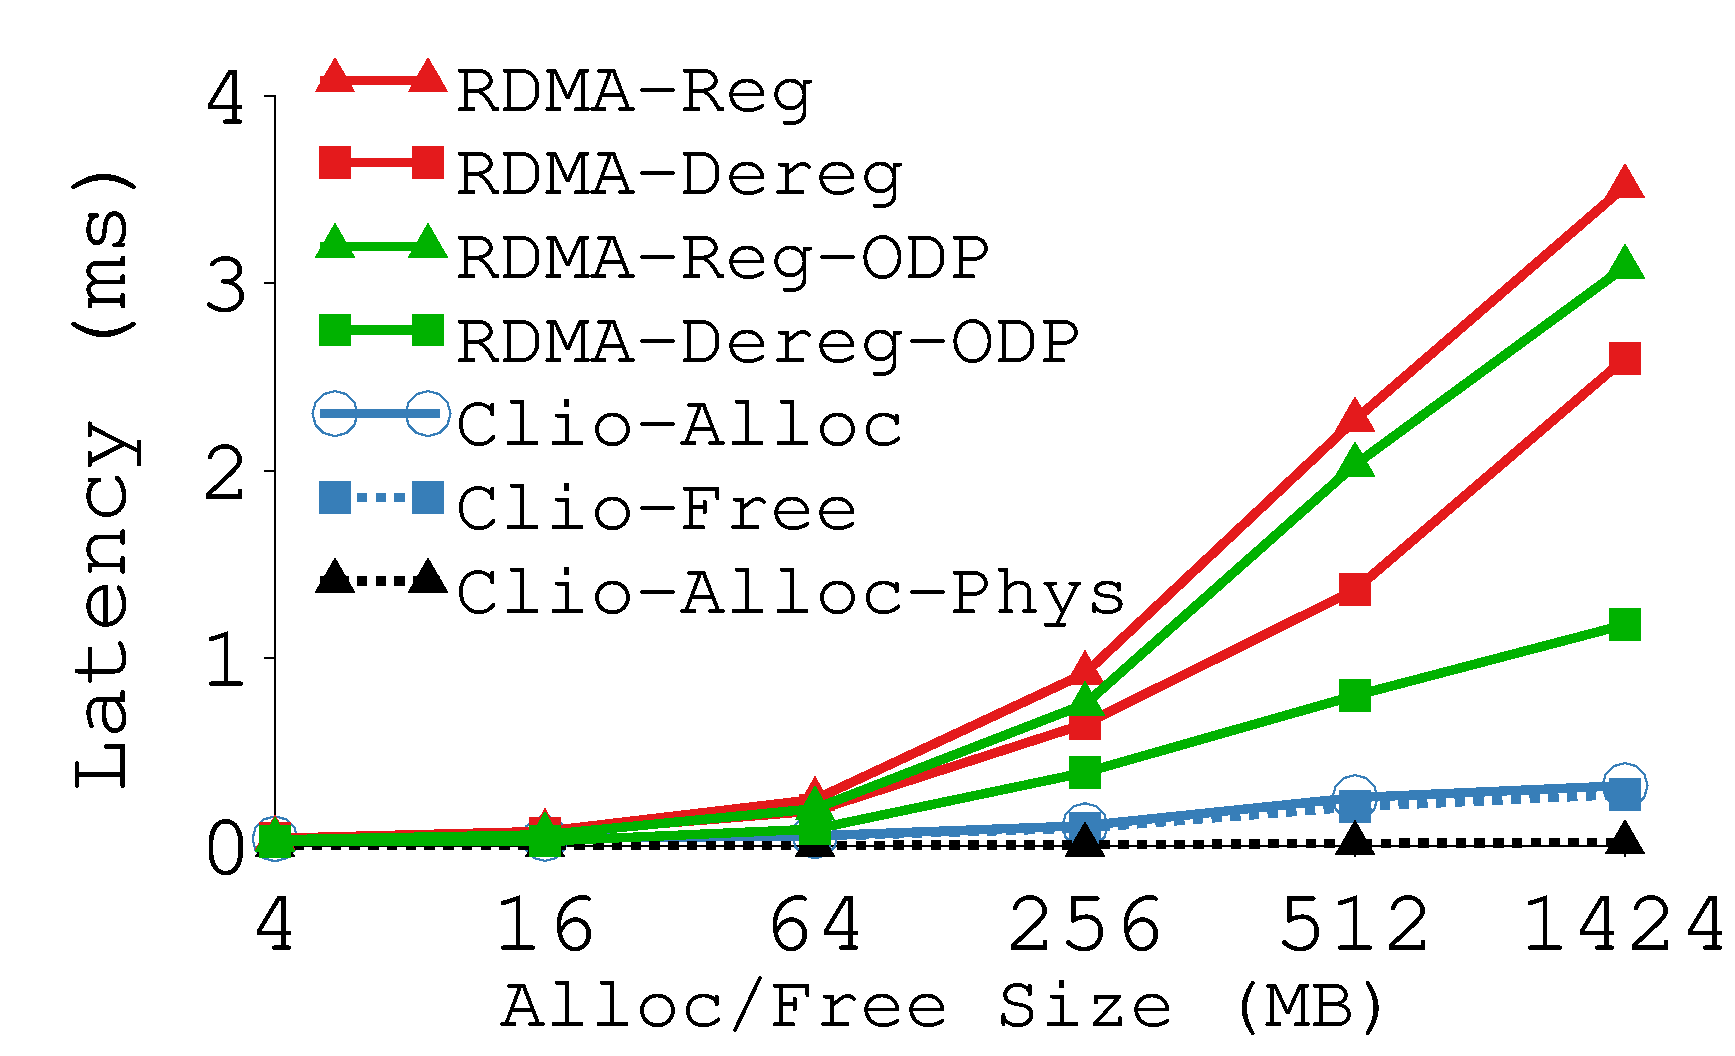
\includegraphics[width=0.5\textwidth]{clio/Figures/g_plot_alloc_free.pdf}}
\mycaption{fig-alloc-free}{Alloc/Free Latency.}
{
ODP means On-Demand-Paging mode
}
\end{center}
\end{figure*}
}
{
\begin{figure*}[h]
\begin{center}
\centerline{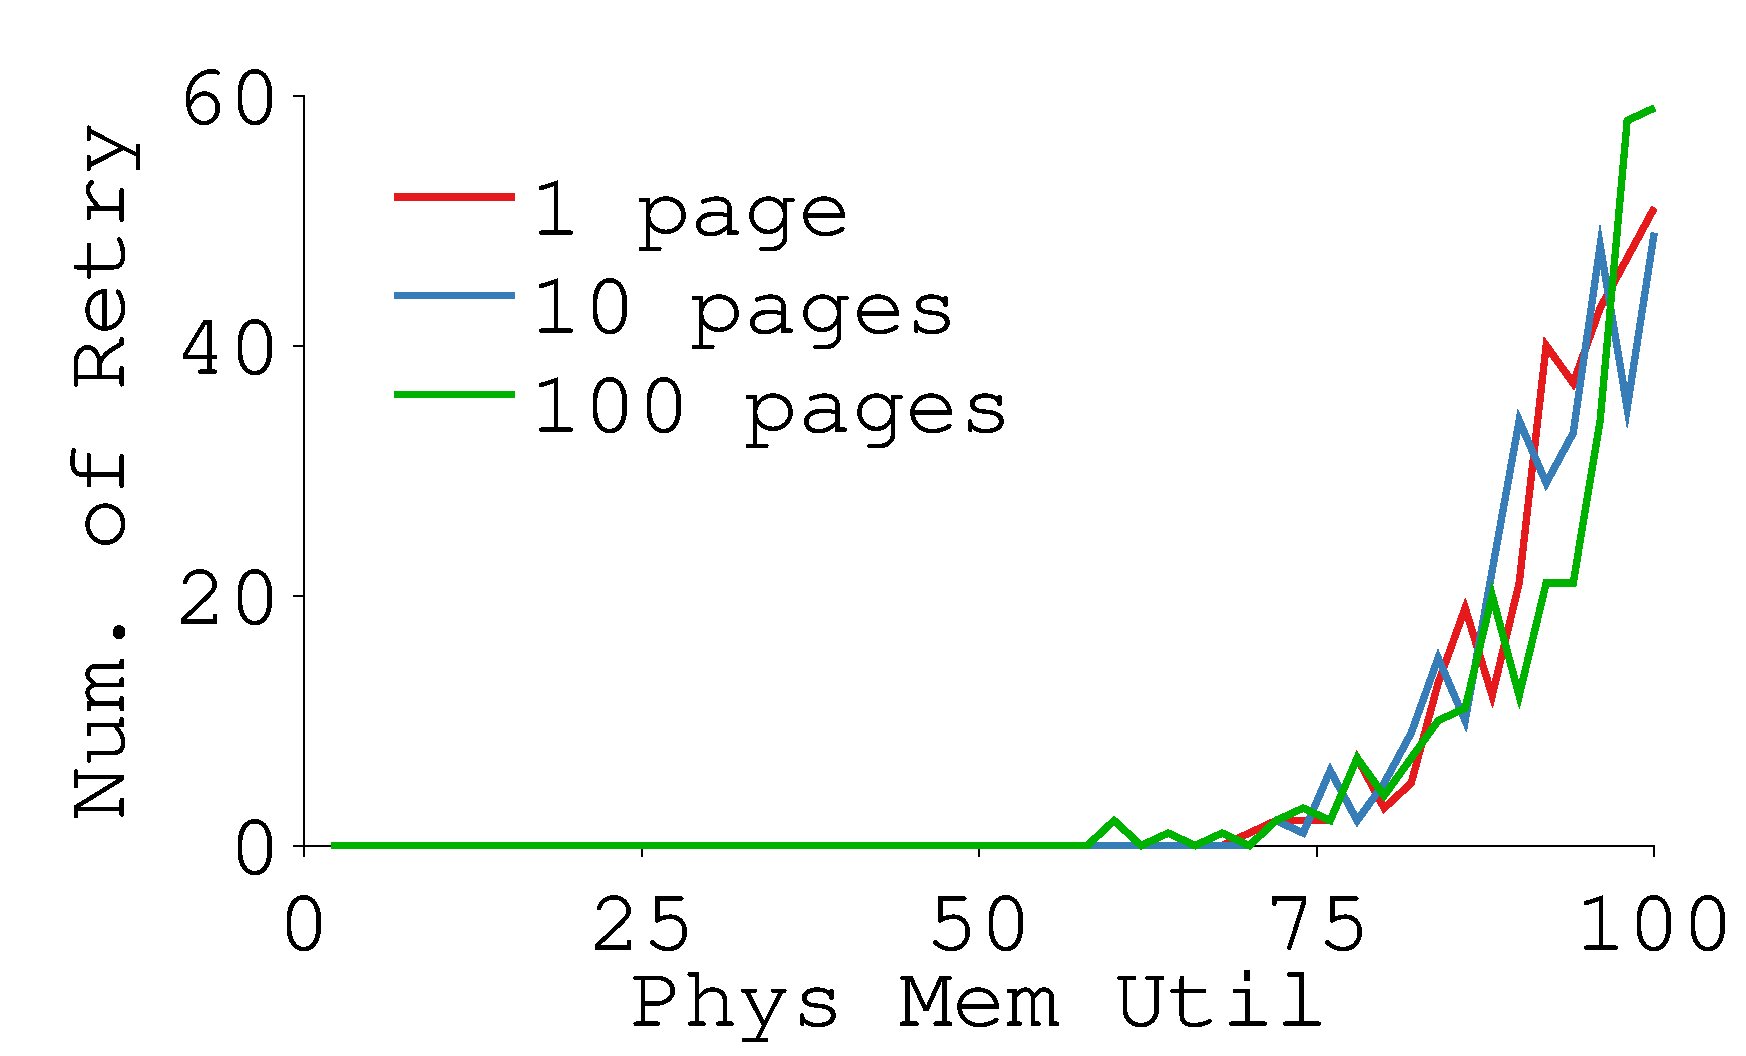
\includegraphics[width=0.5\textwidth]{clio/Figures/g_plot_alloc_conflict.pdf}}
\mycaption{fig-alloc-conflict}{Alloc Retry Rate.}
{
%Alloc's number of retries when vary physical memory utilization.
}
\end{center}
\end{figure*}
}
{
\begin{figure*}[h]
\begin{center}
\centerline{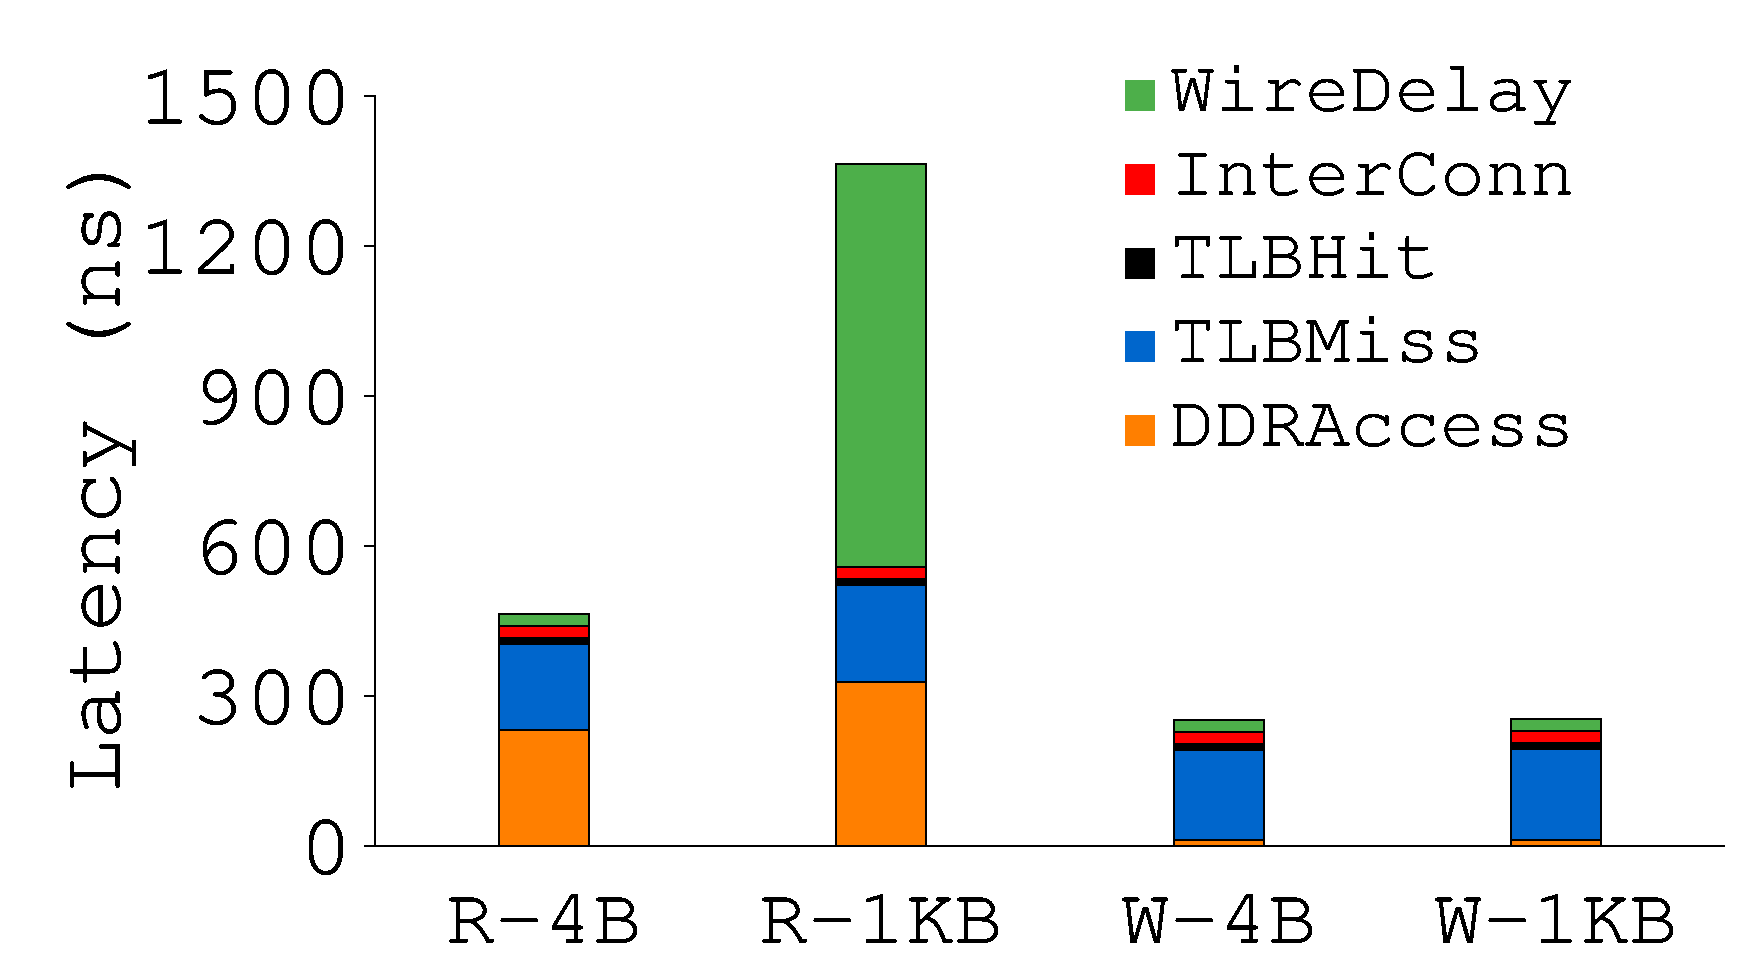
\includegraphics[width=0.5\textwidth]{clio/Figures/g_plot_latency_breakdown.pdf}}
\mycaption{fig-lat-break}{Latency Breakdown.}
{
Breakdown of time spent at \sysboard.
}
\end{center}
\end{figure*}
}
{
\begin{figure*}[h]
\begin{center}
\centerline{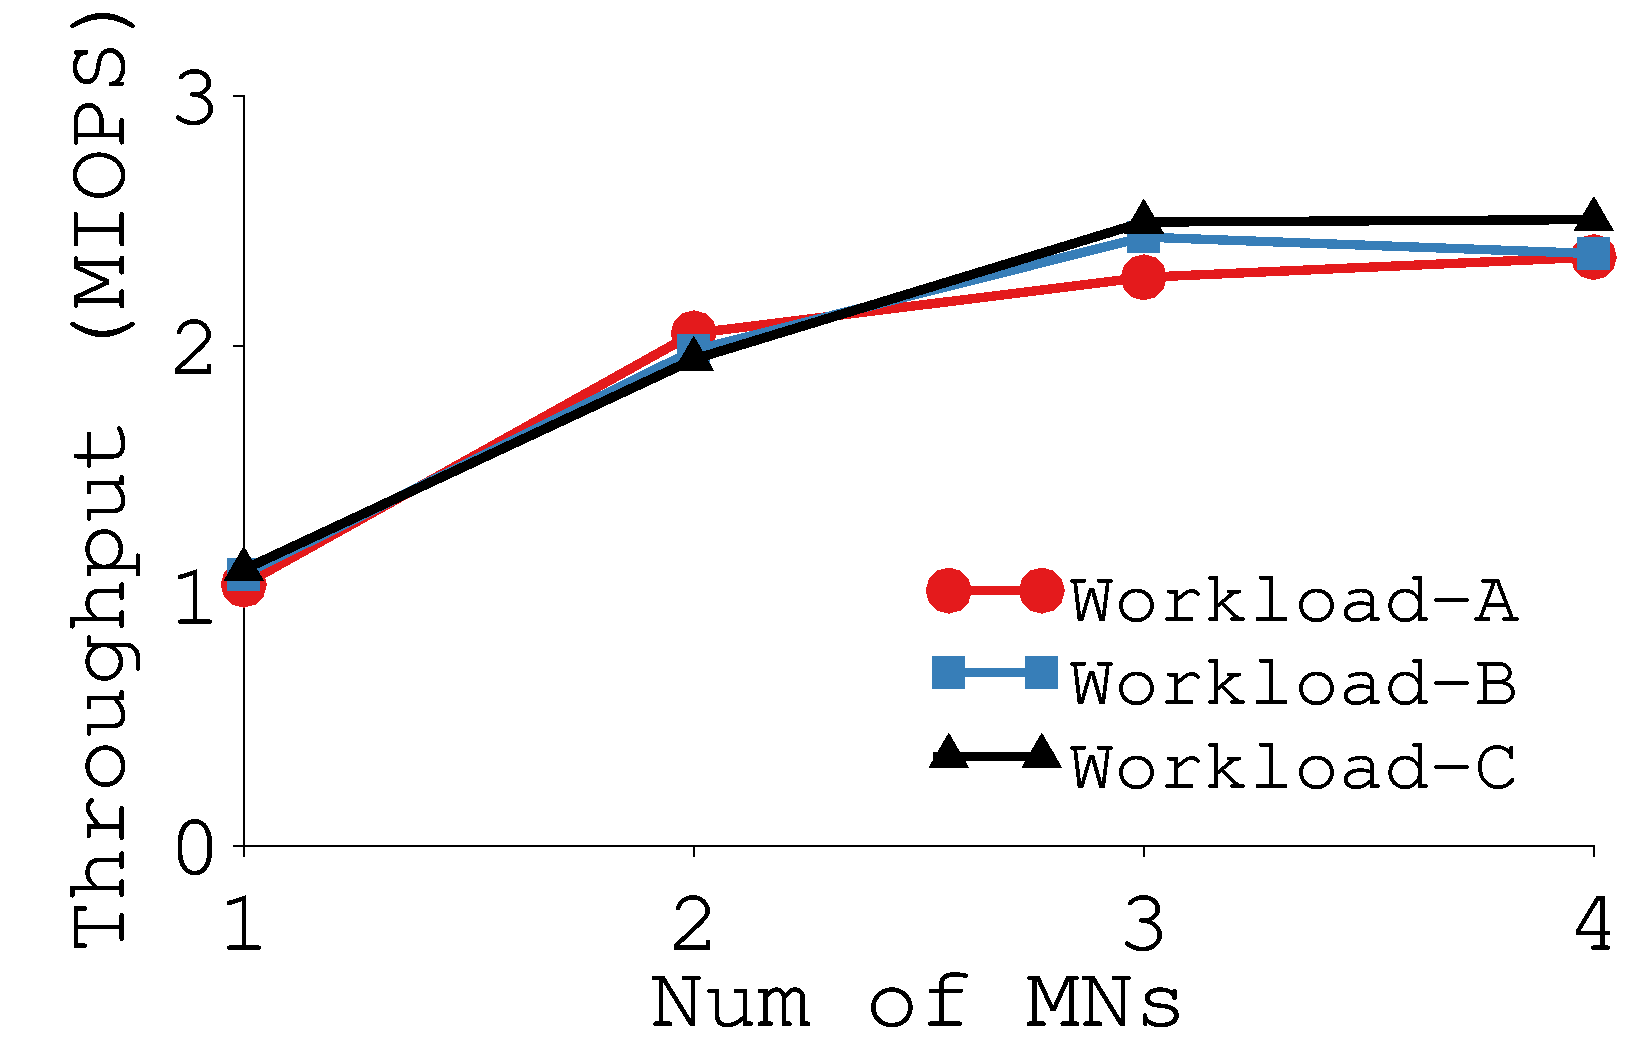
\includegraphics[width=0.5\textwidth]{clio/Figures/g_plot_ycsb_mn.pdf}}
\mycaption{fig-ycsb-mn}{\syskv\ Scalability against \MN{}s.}
{
}
\end{center}
\end{figure*}
}

{
\begin{figure*}[th]
\begin{center}
\centerline{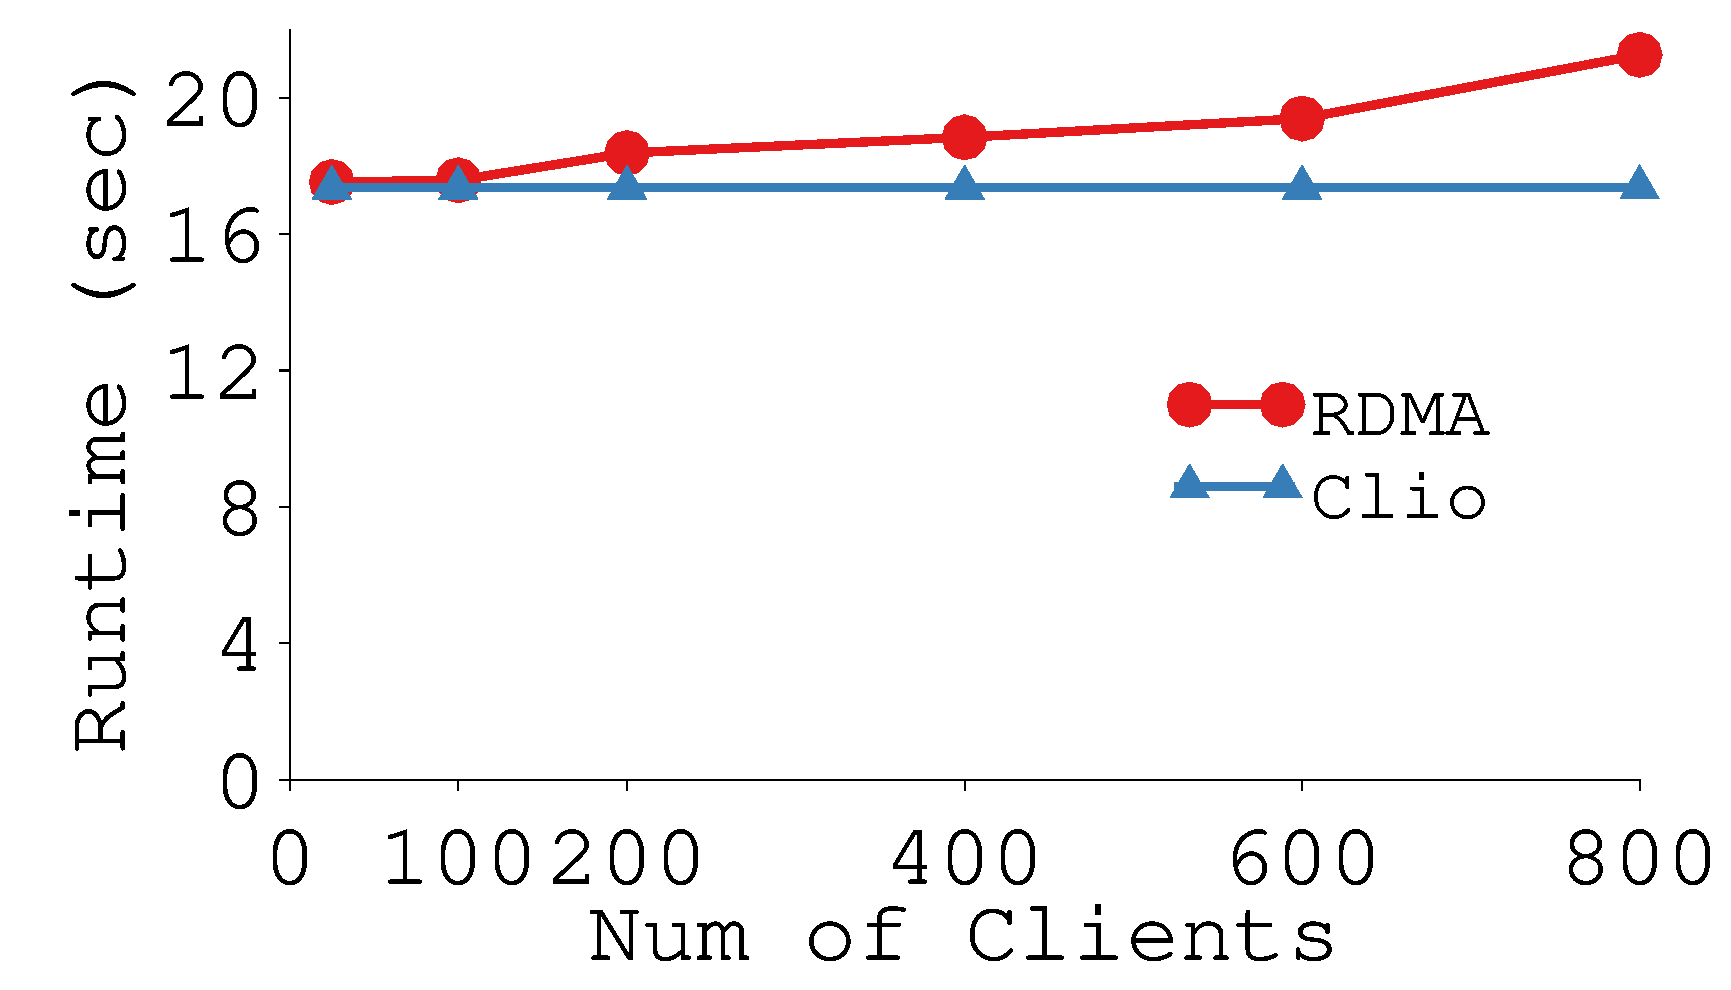
\includegraphics[width=0.5\textwidth]{clio/Figures/g_plot_image_compression.pdf}}
\mycaption{fig-photo}{Image Compression.}
{
}
\end{center}
\end{figure*}
}
{
\begin{figure*}[h]
\begin{center}
\centerline{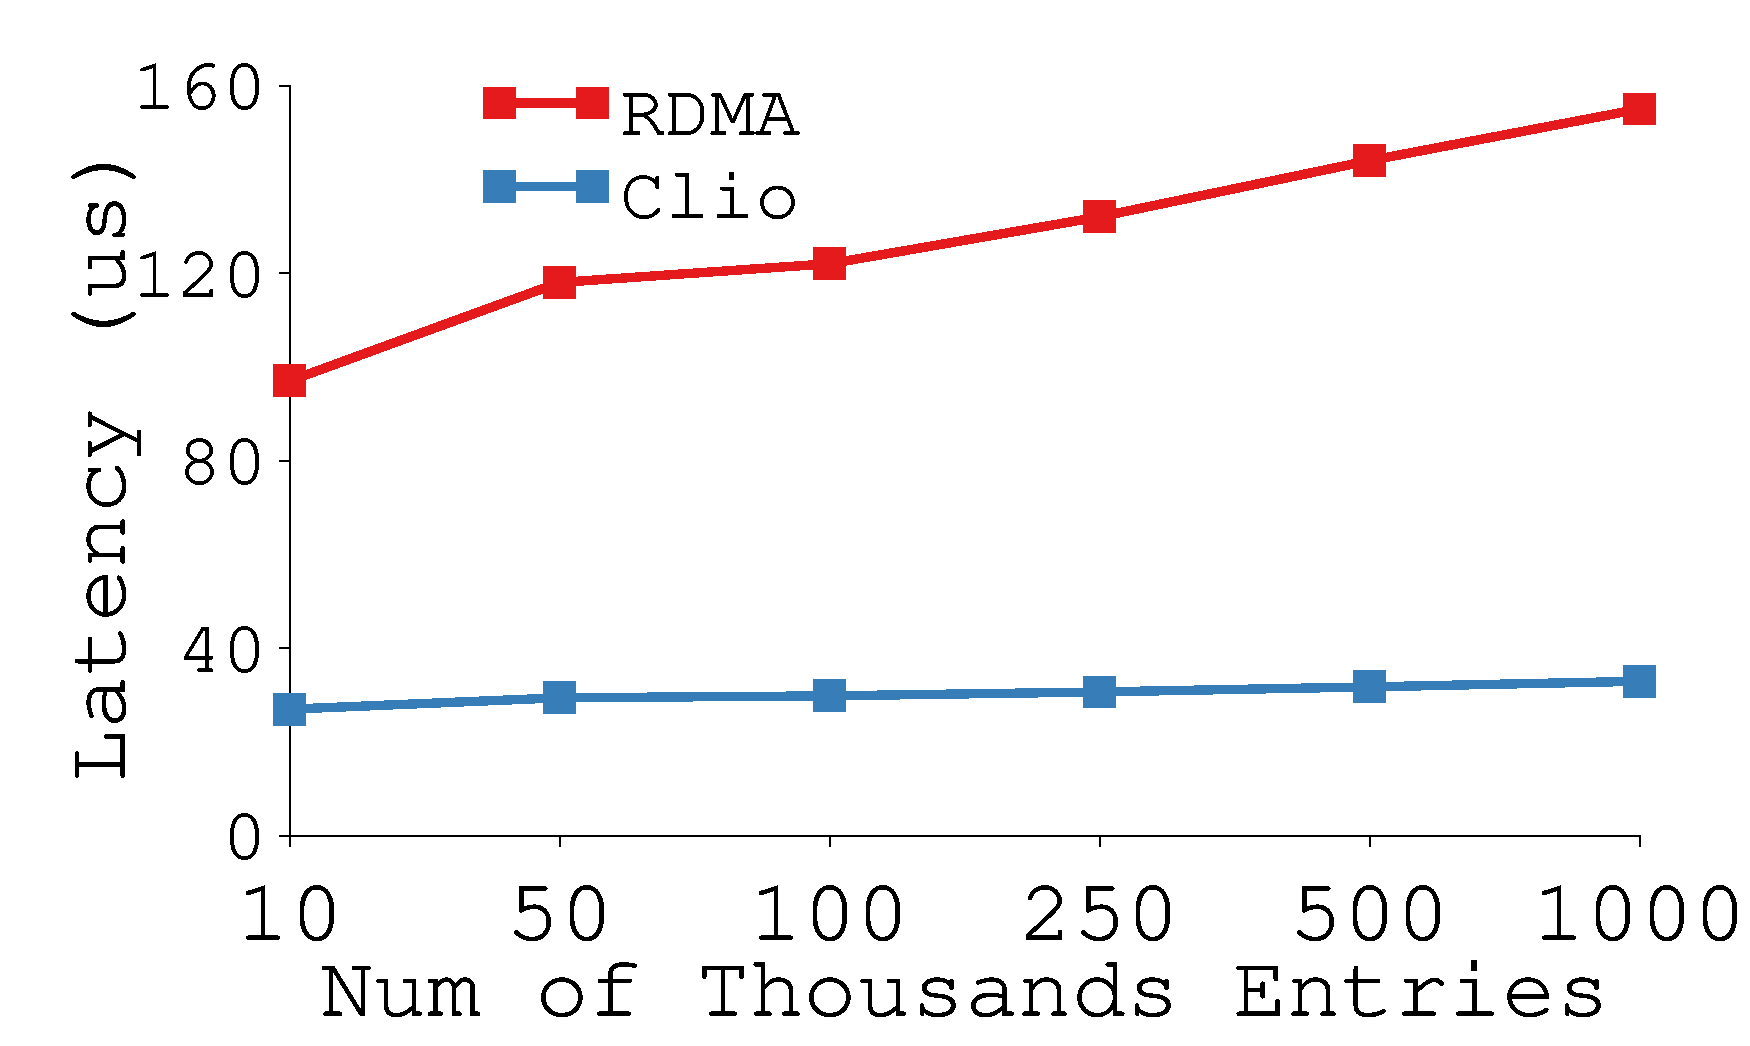
\includegraphics[width=0.5\textwidth]{clio/Figures/g_plot_radix_tree.pdf}}
\mycaption{fig-radix}{Radix Tree Search Latency.}
{
}
\end{center}
\end{figure*}
}
{
\begin{figure*}[h]
\begin{center}
\centerline{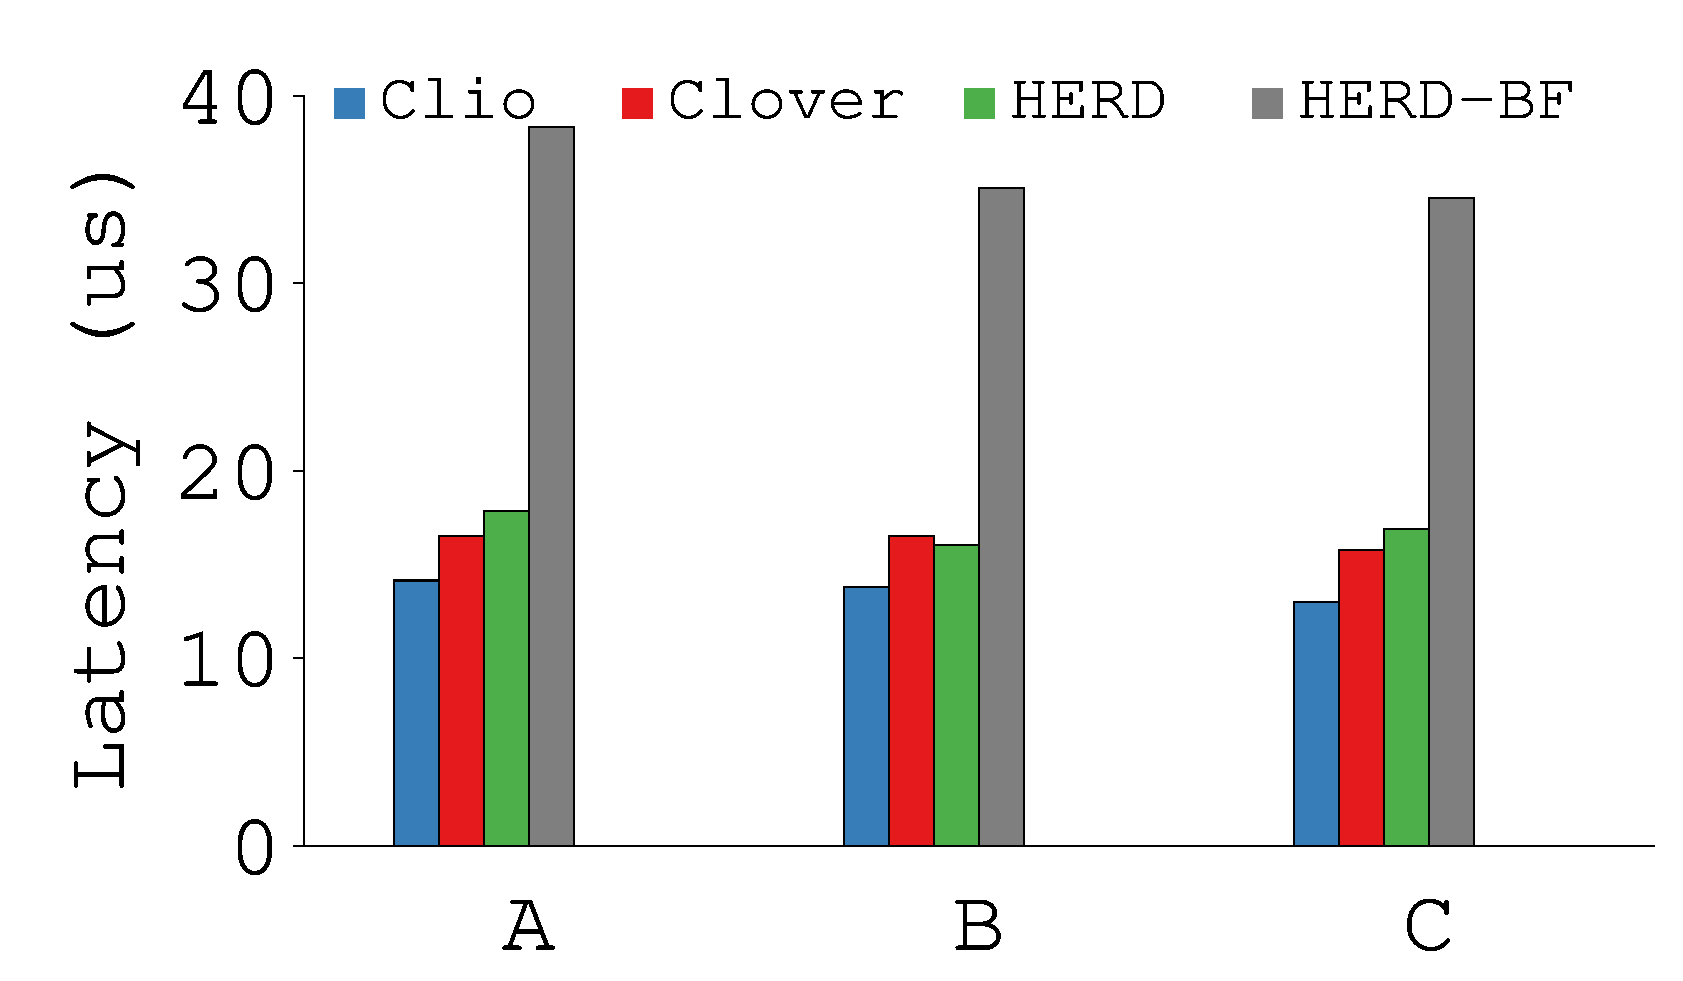
\includegraphics[width=0.5\textwidth]{clio/Figures/g_plot_ycsb_cn.pdf}}
\mycaption{fig-kvstore}{Key-Value Store YCSB Latency.}
{
}
\end{center}
\end{figure*}
}
{
\begin{figure*}[h]
\begin{center}
\centerline{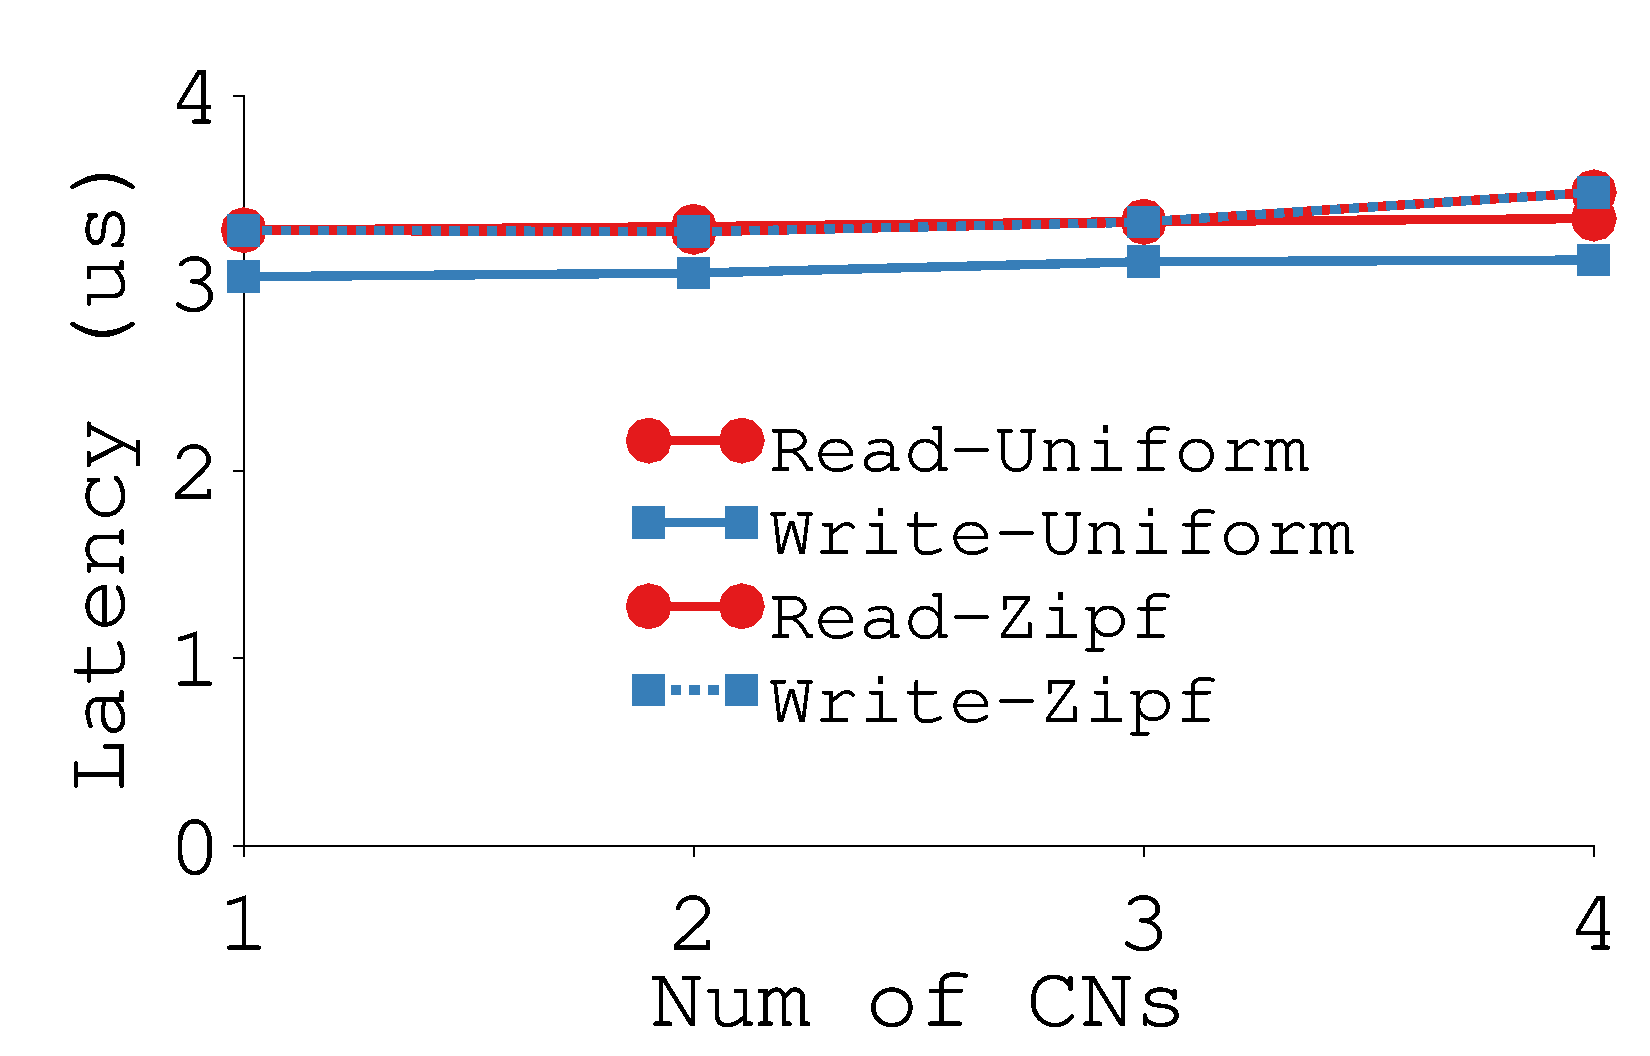
\includegraphics[width=0.5\textwidth]{clio/Figures/g_plot_mvstore.pdf}}
\mycaption{fig-mvstore}{\sysmv\ Object Read/Write Latency.}
{
}
\end{center}
\end{figure*}
}


\ulinebfpara{Scalability.}
We first compare the scalability of \sys\ and RDMA.
Figure~\ref{fig-conn} measures the latency of \sys\ and RDMA as the number of client processes increases.
For RDMA, each process uses its own QP.
Since \sys\ is connectionless, it scales perfectly with the number of processes.
RDMA scales poorly with its QP, and the problem persists with newer generations of RNIC,
which is also confirmed by our previous works~\cite{Pythia,Storm}.

Figure~\ref{fig-pte-mr} evaluates the scalability with respect to PTEs and memory regions.
For the memory region test, we register multiple MRs using the same physical memory for RDMA.
For \sys, we map a large range of VAs (up to 4\TB) to a small physical memory space, as our testbed only has 2\GB\ physical memory.
However, the number of PTEs and the amount of processing needed are the same for \sysboard\ as if it had a real 4\TB\ physical memory.
Thus, this workload stress tests \sysboard's scalability.
%For \sys\ (which gets rid of the MR concept), we use multiple processes to share the same memory,
%resulting in one PTE per process.
RDMA's performance starts to degrade when there are more than $2^8$ (local cluster) or $2^{12}$ (CloudLab),
and the scalability wrt MR is worse than wrt PTE.
In fact, RDMA fails to run beyond $2^{18}$ MRs.
In contrast, \sys\ scales well and never fails (at least up to 4\TB\ memory).
It has two levels of latency that are both stable: a lower latency below $2^4$ for TLB hit and a higher latency above $2^4$ for TLB miss (which always involves one DRAM access).
A \sysboard\ could use a larger TLB if optimal performance is desired.

These experiments confirm that \textbf{\sys\ can handle thousands of concurrent clients and TBs of memory}.



\ulinebfpara{Latency variation.}
Figure~\ref{fig-miss-hit} plots the latency of reading/writing 16\,B data 
when the operation results in a TLB hit, a TLB miss, a first-access page fault, and MR miss (for RDMA only, when the MR metadata is not in RNIC).
RDMA's performance degrades significantly with misses.
Its page fault handling is extremely slow (16.8\ms).
We confirm the same effect on CloudLab with the newer ConnectX-5 NICs.
\sys\ only incurs a small TLB miss cost and \textbf{no additional cost of page fault handling}.

We also include a projection of \sys's latency if it was to be implemented using a real ASIC-based \sysboard.
Specifically, we collect the latency breakdown of time spent on the network wire and at \CN, time spent on third-party FPGA IPs,
number of cycles on FPGA, and time on accessing on-board DRAM.
We maintain the first two parts, scale the FPGA part to ASIC's frequency (2\,GHz), use DDR access time collected on our server to replace the access time to on-board DRAM (which 
goes through a slow board memory controller).
This estimation is conservative, as a real ASIC implementation of the third-party IPs would make the total latency lower.
Our estimated read latency is better than RDMA, while write latency is worse.
We suspect the reason being Nvidia RNIC's optimization of replying a write before it is fully written to DRAM, which \sys\ could also potentially adopt.

Figure~\ref{fig-tail-latency} plots the request latency CDF of continuously running read/write 16\,B data while not triggering page faults.
Even without page faults, \sys\ has much less latency variation and a much shorter tail than RDMA.
%Thanks to our bounded address translation and deterministic hardware design, \sys\ has much less latency variation and a much shorter tail than RDMA.

{
\begin{figure*}[th]
\begin{center}
\centerline{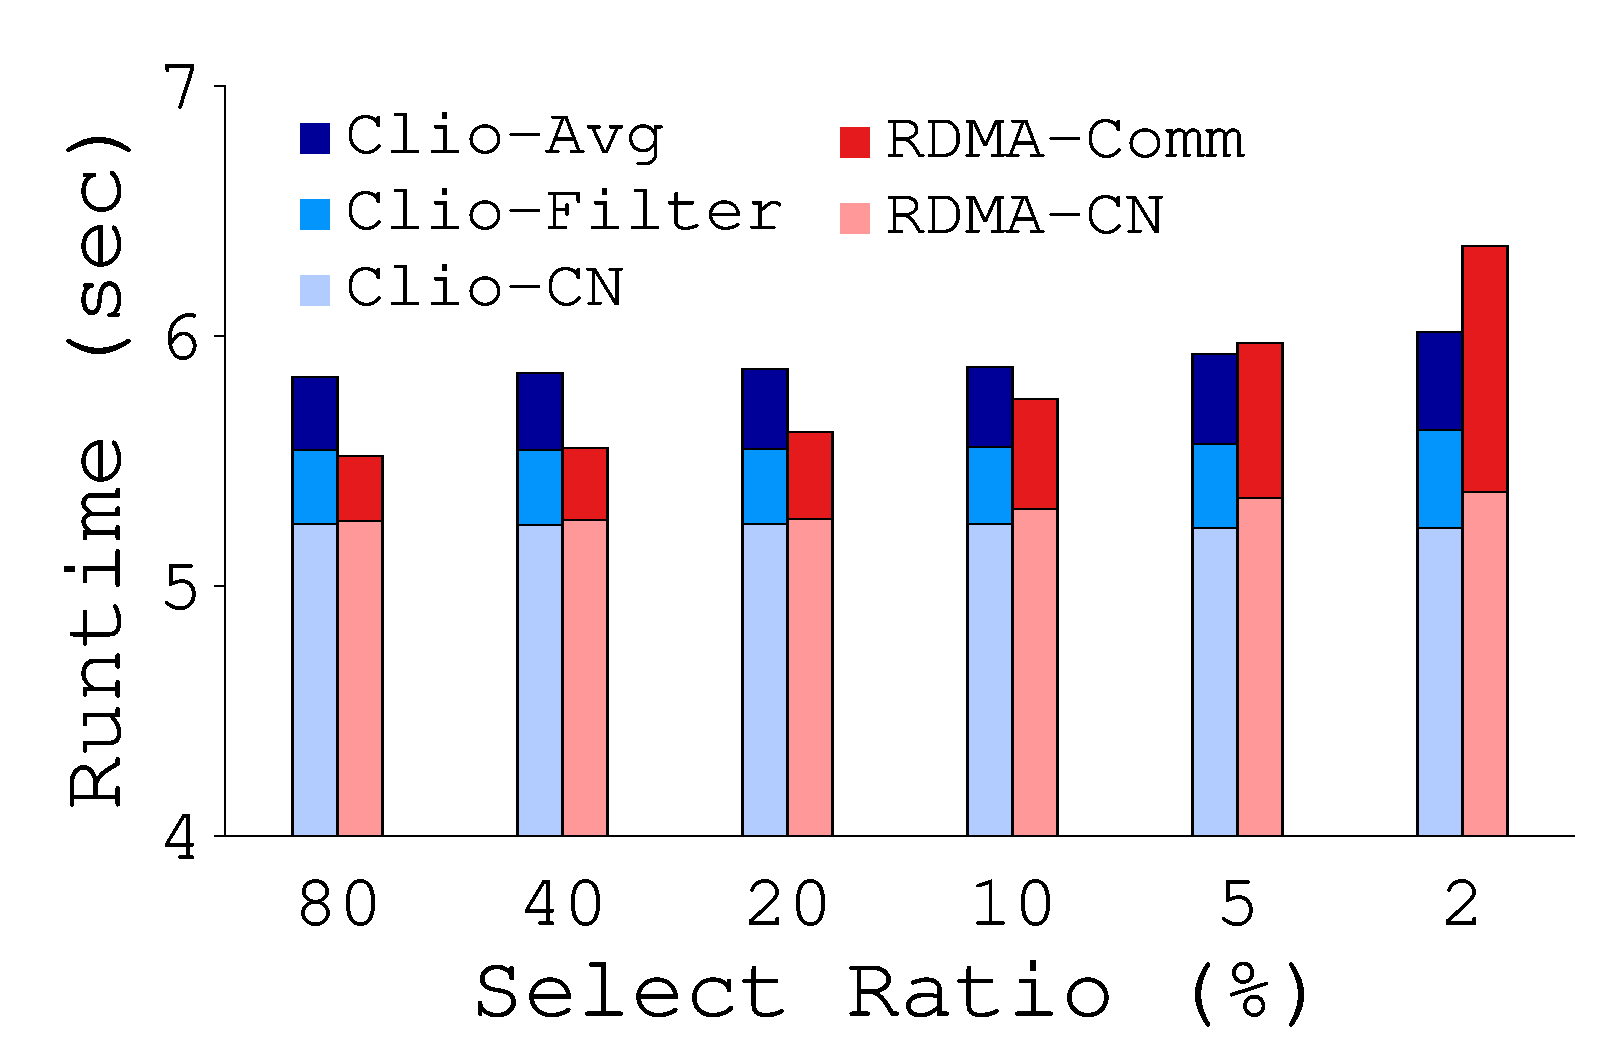
\includegraphics[width=0.5\textwidth]{clio/Figures/g_plot_dp.pdf}}
\mycaption{fig-dataframe}{Select-Aggregate-Shuffle.}
{
Y axis starts at 4 sec. 
CN represents computation done at \CN.
%, as histogram  time is the same.
}
\end{center}
\end{figure*}
}
{
\begin{figure*}[h]
\begin{center}
\centerline{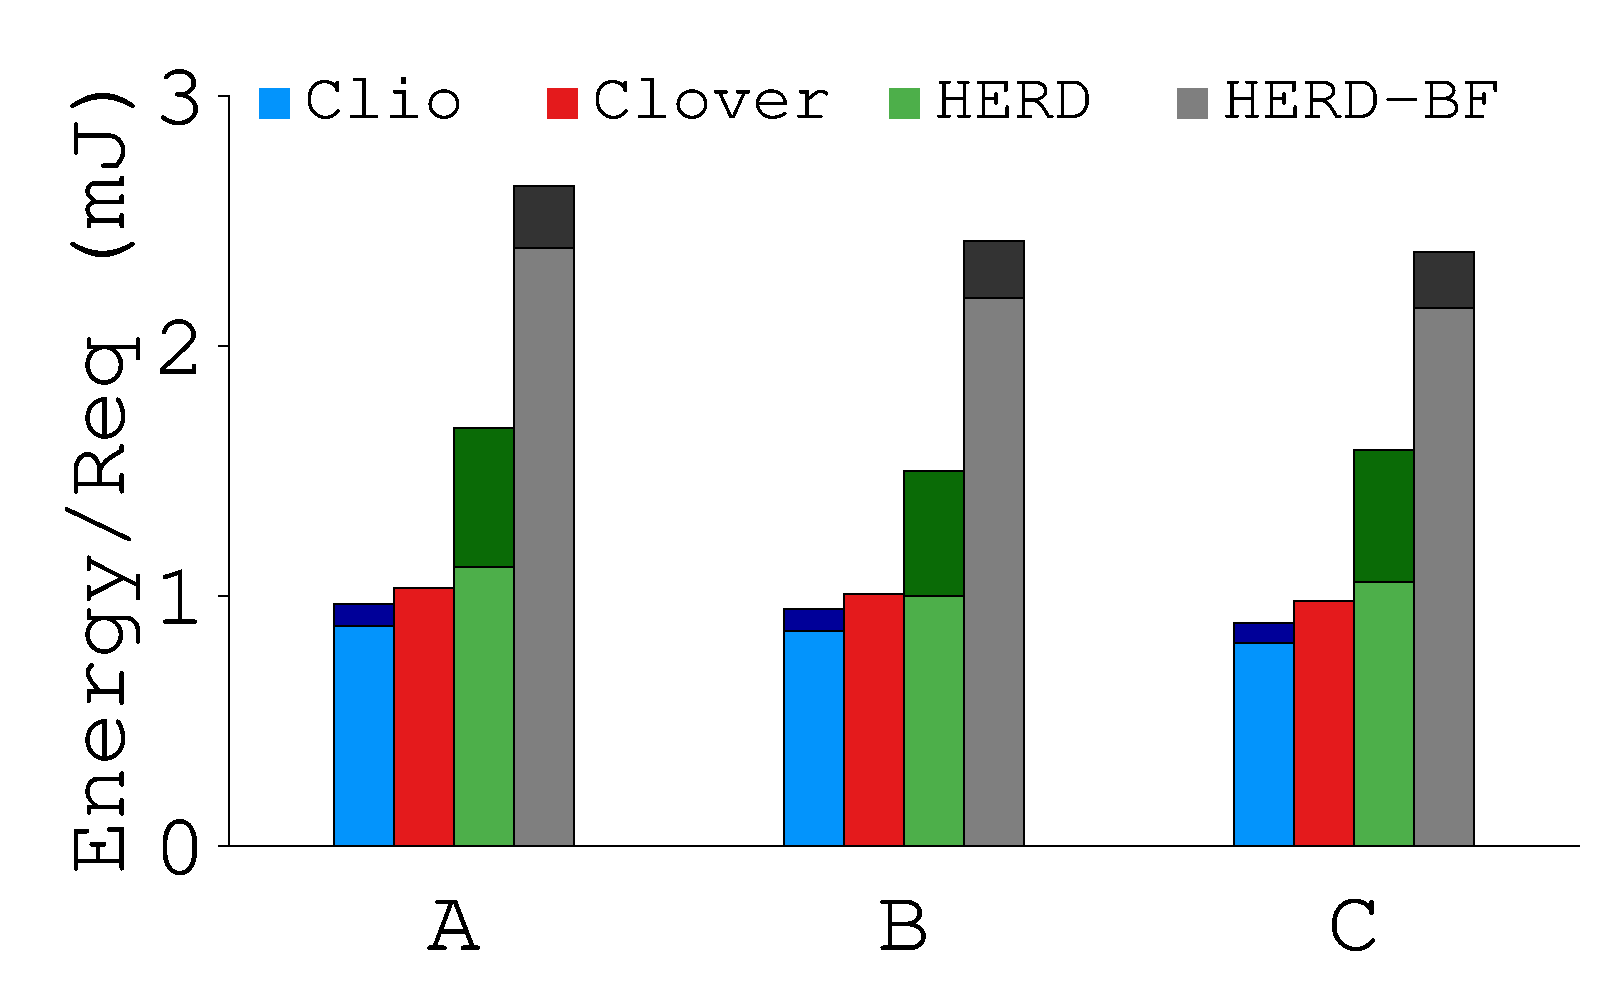
\includegraphics[width=0.5\textwidth]{clio/Figures/g_plot_ycsb_energy.pdf}}
\mycaption{fig-energy}{Energy Comparison.}
{
Darker/lighter shades represent energy spent at \MN{}s and \CN{}s.
}
\end{center}
\end{figure*}
}
{
\begin{table}\small
\begin{center}
\begin{center}
\begin{tabular}{ p{1.2in} | p{0.5in} |p{0.6in} }
 & \textbf{Logic} & \textbf{Memory} \\
\textbf{System/Module} & \textbf{(LUT)} & \textbf{(BRAM)} \\
\hline
\hline
StRoM-RoCEv2 & 39\% & 76\% \\
Tonic-SACK & 48\% & 40\% \\
\hline
\sys\ (Total) & 31\% & 31\% \\
VirtMem & 5.5\% & 3\% \\
NetStack & 2.3\% & 1.7\% \\
\hline
Go-Back-N & 5.8\% & 2.6\% \\
\end{tabular}
\end{center}
\mycaption{fig-fpga-resource}{Clio FPGA Utilization.}
{
}
\end{center}
\end{table}
}

\ulinebfpara{Read/write throughput.}
We measure \sys's throughput by varying the number of concurrent client threads (Figure~\ref{fig-read-write-throughput}).
\sys's default asynchronous APIs quickly reach the line rate of our testbed (9.4\Gbps\ maximum throughput).
Its synchronous APIs could also reach line rate fairly quickly.

Figure~\ref{fig-onboard-throughput} measures the maximum throughput of \sys's FPGA implementation without the bottleneck of the board's 10\Gbps\ port, by generating traffic on board.
Both read and write can reach more than 110\Gbps\ when request size is large.
Read throughput is lower than write when request size is smaller.
We found the throughput bottleneck to be the third-party non-pipelined DMA IP
(which could potentially be improved).

\ulinebfpara{Comparison with other systems.}
We compare \sys\ with native one-sided RDMA, Clover~\cite{Tsai20-ATC}, HERD~\cite{Kalia14-RDMAKV}, and LegoOS~\cite{Shan18-OSDI}.
We ran HERD on both CPU and BlueField (HERD-BF).
%Native RDMA can be considered as a baseline (optimal performance but low-level, restrictive interface).
Clover is a passive disaggregated persistent memory system which we adapted as a passive disaggregated memory (PDM) system.
HERD is an RDMA-based system that supports a key-value interface with an RPC-like architecture.
LegoOS builds its virtual memory system in software at \MN.
%It uses one RDMA read for its read and one RDMA write plus one 
%it can be considered as a software-based active disaggregated memory system. 

\sys's performance is similar to HERD and close to native RDMA.
%\sys's write performance is better than Clover and similar to HERD. %but has a constant overhead over native RDMA.
Clover's write is the worst because it uses at least 2 RTTs for writes to deliver its consistency guarantees without any processing power at \MN{}s.
HERD-BF's latency is much higher than when HERD runs on CPU
due to the slow communication between BlueField's ConnectX-5 chip and ARM processor chip.
LegoOS's latency is almost two times higher than \sys's when request size is small.
In addition, from our experiment, LegoOS can only reach a peak throughput of 77\Gbps, while \sys\ can reach 110\Gbps.
LegoOS' performance overhead comes from its software approach, demonstrating the necessity of a hardware-based solution like \sys.
%due to the slow communication between BlueField's Connect-X5 chip and ARM processor %chip..
%\sys's write overhead can be attributed to \fixme{XXX}.

\ulinebfpara{Allocation performance.}
Figure~\ref{fig-alloc-free} shows \sys's VA and PA allocation and RDMA's MR registration performance.
%Physical memory allocation includes the time to perform an allocation with the buddy algorithm and to insert the allocated address into the free page list.
%It is very fast, indicating that our asynchronous free physical page generation could keep up with most workloads' page fault speed.
%Virtual memory allocation and free (measured from client on \CN) are slower,
\sys's PA allocation takes less than 20\mus, and the VA allocation is much faster than RDMA MR registration,
although both get slower with larger allocation/registration size.
%since these operations involve the costly crossing between FPGA and ARM.
%They are also slower with larger sizes, as searching the VMA tree for a big free region takes more time.
Figure~\ref{fig-alloc-conflict} shows the number of retries at allocation time with three allocation sizes as the physical memory fills up.
%running at on-board ARM processor.
%The hash-based page table is proportional to the physical memory size. 
%Hence higher its utilization, higher the overflow probability therefore higher number of retries.
%The page table has 2\x\ extra slots by default.
There is no retry when memory is below half utilized. Even when memory is close to full, there are at most 60 retries per allocation request, with roughly 0.5\ms\ per retry. This confirms that our design of avoiding hash overflows at allocation time is practical.
%co-design of overflow-free hash-based page table and allocation retry scheme is practical.


\ulinebfpara{Close look at \sysboard{} components.}
To further understand \sys's performance, % and to determine the reason for worse large-read performance,
we profile different parts of \sys's processing for read and write of 4\,B to 1\KB.
\syslib\ adds a very small overhead (250\ns\ in total), 
thanks to our efficient threading model and network stack implementation.
Figure~\ref{fig-lat-break} shows the latency breakdown at \sysboard.
Time to fetch data from DRAM (DDRAccess) and to transfer it over the wire (WireDelay) are the main 
contributor to read latency, especially with large read size.
Both could be largely improved in a real \sysboard\ with better memory controller and higher frequency.
TLB miss (which takes one DRAM read) is the other main part of the latencies.


\subsection{Application Performance}

\ulinebfpara{Image Compression.}
We run a workload where each client 
compresses and decompresses 1000 256*256-pixel images with increasing number of concurrently running clients.
Figure~\ref{fig-photo} shows the total runtime per client.
We compare \sys\ with RDMA, with both performing computation at the \CN\ side and the RDMA using one-sided operations instead of \sys\ APIs to read/write images in remote memory.
\sys's performance stays the same as the number of clients increase.
RDMA's performance does not scale because it requires each client to register a different MR to have protected memory accesses.
With more MRs, RDMA runs into the case where the RNIC cannot hold all the MR metadata and many accesses would involve a slow read to host main memory.

\ulinebfpara{Radix Tree.}
Figure~\ref{fig-radix} shows the latency of searching a key in pre-populated radix trees when varying the tree size. 
We again compare with RDMA which uses one-sided read operations to perform the tree traversal task.
RDMA's performance is worse than \sys,
because it requires multiple RTTs to traverse the tree,
while \sys\ only needs one RTT for each pointer chasing (each tree level).
In addition, RDMA also scales worse than \sys.

\ulinebfpara{Key-value store.}
Figure~\ref{fig-kvstore} evaluates \syskv\ using the YCSB benchmark~\cite{YCSB} and compares it to Clover, HERD, and HERD-BF.
We run two \CN{}s and 8 threads per \CN.
We use 100K key-value entries and run 100K operations per test,
with YCSB's default key-value size of 1\KB. %where the key size is 8 bytes and the value size is 1\KB.
The accesses to keys follow the Zipf distribution ($\theta=0.99$).
We use three YCSB workloads with different {\em get-set} ratios: 
100\% {\em get} (workload C), 5\% {\em set} (B), and 50\% {\em set} (A).
\syskv\ performs the best.
HERD running on BlueField performs the worst, mainly because BlueField's slower crossing between its NIC chip and ARM chip.




Figures~\ref{fig-ycsb-mn} shows the throughput of \syskv\ when varying the number of MNs. Similar to our
\sys\ scalability results, \syskv\ can reach a CN’s maximum
throughput and can handle concurrent get/set requests even
under contention. These results are similar to or better than
previous FPGA-based and RDMA-based key-value stores that
are fine-tuned for just key-value workloads (Table 3 in \cite{KVDIRECT}),
while we got our results without any performance tuning.

\ulinebfpara{Multi-version data store.}
%\subsubsection{Multi-Version Data Store}
We evaluate \sysmv\ by varying the number of \CN{}s that concurrently access data objects (of 16\,B) on an \MN\ using workloads of 50\% read (of different versions) and 50\% write under uniform and Zipf distribution of objects (Figure~\ref{fig-mvstore}). 
\sysmv's read and write have the same performance, and reading any version has the 
same performance, since we use an array-based version design. 
%Running multiple \MN{}s have similar performance and we omit for space.




\ulinebfpara{Data analytics.}
We run a simple workload which first \texttt{select} rows in a table whose field-A matches a value (\eg, gender is female)
and calculate \texttt{avg} of field-B (\eg, final score) of all the rows.
Finally, it calculates the histogram of the selected rows (\eg, score distribution), which can be presented to the user together with the avg value. %(\eg, how female students' scores compare to the whole class).
\sys\ executes the first two steps at \MN\ offloads and the final step at \CN,
while RDMA always reads rows to \CN\ and then does each operation.
Figure~\ref{fig-dataframe} plots the total run time as the select ratio decreases (fewer rows selected).
% When the select ratio is high, \sys\ and RDMA send a similar amount of data across the network,
% and as the CPU computation is faster than our FPGA implementation for these operations, \sys's overall performance is worse than RDMA.
When the select ratio is low, \sys\ transfers much less data than RDMA, resulting in its better performance.




%To put \sys\ in respective with other existing RDMA-based and FPGA-based key-value stores that we couldn't directly compare with (\eg, close-sourced), we compare 
%\syskv's latency results with reported latencies in ~\cite{KVDIRECT}. 
%\syskv\ has {\bf lower end-to-end latency than all these existing systems}.

%then sends the data to \CN, which shuffles the data and sends the shuffled 
%data back to \MN\ for aggregation.

\subsection{CapEx, Energy, and FPGA Utilization}
\label{sec:clio:results-cost}


We estimate the cost of server and \sysboard\ using market prices of different hardware units. When using 1\TB\ DRAM, a server-based \MN\ costs 1.1-1.5\x\ and consumes 1.9-2.7\x\ power compared to \sysboard. These numbers become 1.4-2.5\x\ and 5.1-8.6\x\ with OptaneDimm~\cite{optane-dcpm}, which we expect to be the more likely remote memory media in future systems.


We measure the total energy used for running YCSB workloads
by collecting the total CPU (or FPGA) cycles and the Watt of a CPU core~\cite{gold5128}, ARM processor~\cite{armpower}, and FPGA (measured).
We omit the energy used by DRAM and NICs in all the calculations. 
Clover, a system that centers its design around low cost, has slightly higher energy than \sys.
Even though there is no processing at \MN{}s for Clover, its \CN{}s use more cycles to process and manage memory.
HERD consumes 1.6\x\ to 3\x\ more energy than \sys, mainly because of its CPU overhead at \MN{}s.
Surprisingly, HERD-BF consumes the most energy, even though it is a low-power ARM-based SmartNIC.
This is because of its worse performance and longer total runtime.

Figure~\ref{fig-fpga-resource} compares the FPGA utilization among Clio, StRoM's RoCEv2~\cite{StRoM}, and Tonic's selective ack stack~\cite{TONIC}.
%With our design that is tailored to save resources, 
%\sys\ consumes roughly one third of the total resources.
Both StRoM and Tonic include only a network stack but they consume more resources than \sys.
Within \sys, the virtual memory (VirtMem) and
the network stack (NetStack) consume a small fraction of the total resources,
with the rest being vendor IPs (PHY, MAC, DDR4, and interconnect).
%To put things in perspective, we implement a Go-back-N network stack which supports 1K connections. It uses 2.5\x\ more logic than what our current network stack consumes. 
Overall, our efficient hardware implementation leaves most FPGA resources available for application offloads.
